\documentclass{article}
\usepackage{iclr2025,times}

% Optional math commands
%%%%% NEW MATH DEFINITIONS %%%%%

\usepackage{amsmath,amsfonts,bm}

% Mark sections of captions for referring to divisions of figures
\newcommand{\figleft}{{\em (Left)}}
\newcommand{\figcenter}{{\em (Center)}}
\newcommand{\figright}{{\em (Right)}}
\newcommand{\figtop}{{\em (Top)}}
\newcommand{\figbottom}{{\em (Bottom)}}
\newcommand{\captiona}{{\em (a)}}
\newcommand{\captionb}{{\em (b)}}
\newcommand{\captionc}{{\em (c)}}
\newcommand{\captiond}{{\em (d)}}

% Highlight a newly defined term
\newcommand{\newterm}[1]{{\bf #1}}


% Figure reference, lower-case.
\def\figref#1{figure~\ref{#1}}
% Figure reference, capital. For start of sentence
\def\Figref#1{Figure~\ref{#1}}
\def\twofigref#1#2{figures \ref{#1} and \ref{#2}}
\def\quadfigref#1#2#3#4{figures \ref{#1}, \ref{#2}, \ref{#3} and \ref{#4}}
% Section reference, lower-case.
\def\secref#1{section~\ref{#1}}
% Section reference, capital.
\def\Secref#1{Section~\ref{#1}}
% Reference to two sections.
\def\twosecrefs#1#2{sections \ref{#1} and \ref{#2}}
% Reference to three sections.
\def\secrefs#1#2#3{sections \ref{#1}, \ref{#2} and \ref{#3}}
% Reference to an equation, lower-case.
\def\eqref#1{equation~\ref{#1}}
% Reference to an equation, upper case
\def\Eqref#1{Equation~\ref{#1}}
% A raw reference to an equation---avoid using if possible
\def\plaineqref#1{\ref{#1}}
% Reference to a chapter, lower-case.
\def\chapref#1{chapter~\ref{#1}}
% Reference to an equation, upper case.
\def\Chapref#1{Chapter~\ref{#1}}
% Reference to a range of chapters
\def\rangechapref#1#2{chapters\ref{#1}--\ref{#2}}
% Reference to an algorithm, lower-case.
\def\algref#1{algorithm~\ref{#1}}
% Reference to an algorithm, upper case.
\def\Algref#1{Algorithm~\ref{#1}}
\def\twoalgref#1#2{algorithms \ref{#1} and \ref{#2}}
\def\Twoalgref#1#2{Algorithms \ref{#1} and \ref{#2}}
% Reference to a part, lower case
\def\partref#1{part~\ref{#1}}
% Reference to a part, upper case
\def\Partref#1{Part~\ref{#1}}
\def\twopartref#1#2{parts \ref{#1} and \ref{#2}}

\def\ceil#1{\lceil #1 \rceil}
\def\floor#1{\lfloor #1 \rfloor}
\def\1{\bm{1}}
\newcommand{\train}{\mathcal{D}}
\newcommand{\valid}{\mathcal{D_{\mathrm{valid}}}}
\newcommand{\test}{\mathcal{D_{\mathrm{test}}}}

\def\eps{{\epsilon}}


% Random variables
\def\reta{{\textnormal{$\eta$}}}
\def\ra{{\textnormal{a}}}
\def\rb{{\textnormal{b}}}
\def\rc{{\textnormal{c}}}
\def\rd{{\textnormal{d}}}
\def\re{{\textnormal{e}}}
\def\rf{{\textnormal{f}}}
\def\rg{{\textnormal{g}}}
\def\rh{{\textnormal{h}}}
\def\ri{{\textnormal{i}}}
\def\rj{{\textnormal{j}}}
\def\rk{{\textnormal{k}}}
\def\rl{{\textnormal{l}}}
% rm is already a command, just don't name any random variables m
\def\rn{{\textnormal{n}}}
\def\ro{{\textnormal{o}}}
\def\rp{{\textnormal{p}}}
\def\rq{{\textnormal{q}}}
\def\rr{{\textnormal{r}}}
\def\rs{{\textnormal{s}}}
\def\rt{{\textnormal{t}}}
\def\ru{{\textnormal{u}}}
\def\rv{{\textnormal{v}}}
\def\rw{{\textnormal{w}}}
\def\rx{{\textnormal{x}}}
\def\ry{{\textnormal{y}}}
\def\rz{{\textnormal{z}}}

% Random vectors
\def\rvepsilon{{\mathbf{\epsilon}}}
\def\rvtheta{{\mathbf{\theta}}}
\def\rva{{\mathbf{a}}}
\def\rvb{{\mathbf{b}}}
\def\rvc{{\mathbf{c}}}
\def\rvd{{\mathbf{d}}}
\def\rve{{\mathbf{e}}}
\def\rvf{{\mathbf{f}}}
\def\rvg{{\mathbf{g}}}
\def\rvh{{\mathbf{h}}}
\def\rvu{{\mathbf{i}}}
\def\rvj{{\mathbf{j}}}
\def\rvk{{\mathbf{k}}}
\def\rvl{{\mathbf{l}}}
\def\rvm{{\mathbf{m}}}
\def\rvn{{\mathbf{n}}}
\def\rvo{{\mathbf{o}}}
\def\rvp{{\mathbf{p}}}
\def\rvq{{\mathbf{q}}}
\def\rvr{{\mathbf{r}}}
\def\rvs{{\mathbf{s}}}
\def\rvt{{\mathbf{t}}}
\def\rvu{{\mathbf{u}}}
\def\rvv{{\mathbf{v}}}
\def\rvw{{\mathbf{w}}}
\def\rvx{{\mathbf{x}}}
\def\rvy{{\mathbf{y}}}
\def\rvz{{\mathbf{z}}}

% Elements of random vectors
\def\erva{{\textnormal{a}}}
\def\ervb{{\textnormal{b}}}
\def\ervc{{\textnormal{c}}}
\def\ervd{{\textnormal{d}}}
\def\erve{{\textnormal{e}}}
\def\ervf{{\textnormal{f}}}
\def\ervg{{\textnormal{g}}}
\def\ervh{{\textnormal{h}}}
\def\ervi{{\textnormal{i}}}
\def\ervj{{\textnormal{j}}}
\def\ervk{{\textnormal{k}}}
\def\ervl{{\textnormal{l}}}
\def\ervm{{\textnormal{m}}}
\def\ervn{{\textnormal{n}}}
\def\ervo{{\textnormal{o}}}
\def\ervp{{\textnormal{p}}}
\def\ervq{{\textnormal{q}}}
\def\ervr{{\textnormal{r}}}
\def\ervs{{\textnormal{s}}}
\def\ervt{{\textnormal{t}}}
\def\ervu{{\textnormal{u}}}
\def\ervv{{\textnormal{v}}}
\def\ervw{{\textnormal{w}}}
\def\ervx{{\textnormal{x}}}
\def\ervy{{\textnormal{y}}}
\def\ervz{{\textnormal{z}}}

% Random matrices
\def\rmA{{\mathbf{A}}}
\def\rmB{{\mathbf{B}}}
\def\rmC{{\mathbf{C}}}
\def\rmD{{\mathbf{D}}}
\def\rmE{{\mathbf{E}}}
\def\rmF{{\mathbf{F}}}
\def\rmG{{\mathbf{G}}}
\def\rmH{{\mathbf{H}}}
\def\rmI{{\mathbf{I}}}
\def\rmJ{{\mathbf{J}}}
\def\rmK{{\mathbf{K}}}
\def\rmL{{\mathbf{L}}}
\def\rmM{{\mathbf{M}}}
\def\rmN{{\mathbf{N}}}
\def\rmO{{\mathbf{O}}}
\def\rmP{{\mathbf{P}}}
\def\rmQ{{\mathbf{Q}}}
\def\rmR{{\mathbf{R}}}
\def\rmS{{\mathbf{S}}}
\def\rmT{{\mathbf{T}}}
\def\rmU{{\mathbf{U}}}
\def\rmV{{\mathbf{V}}}
\def\rmW{{\mathbf{W}}}
\def\rmX{{\mathbf{X}}}
\def\rmY{{\mathbf{Y}}}
\def\rmZ{{\mathbf{Z}}}

% Elements of random matrices
\def\ermA{{\textnormal{A}}}
\def\ermB{{\textnormal{B}}}
\def\ermC{{\textnormal{C}}}
\def\ermD{{\textnormal{D}}}
\def\ermE{{\textnormal{E}}}
\def\ermF{{\textnormal{F}}}
\def\ermG{{\textnormal{G}}}
\def\ermH{{\textnormal{H}}}
\def\ermI{{\textnormal{I}}}
\def\ermJ{{\textnormal{J}}}
\def\ermK{{\textnormal{K}}}
\def\ermL{{\textnormal{L}}}
\def\ermM{{\textnormal{M}}}
\def\ermN{{\textnormal{N}}}
\def\ermO{{\textnormal{O}}}
\def\ermP{{\textnormal{P}}}
\def\ermQ{{\textnormal{Q}}}
\def\ermR{{\textnormal{R}}}
\def\ermS{{\textnormal{S}}}
\def\ermT{{\textnormal{T}}}
\def\ermU{{\textnormal{U}}}
\def\ermV{{\textnormal{V}}}
\def\ermW{{\textnormal{W}}}
\def\ermX{{\textnormal{X}}}
\def\ermY{{\textnormal{Y}}}
\def\ermZ{{\textnormal{Z}}}

% Vectors
\def\vzero{{\bm{0}}}
\def\vone{{\bm{1}}}
\def\vmu{{\bm{\mu}}}
\def\vtheta{{\bm{\theta}}}
\def\va{{\bm{a}}}
\def\vb{{\bm{b}}}
\def\vc{{\bm{c}}}
\def\vd{{\bm{d}}}
\def\ve{{\bm{e}}}
\def\vf{{\bm{f}}}
\def\vg{{\bm{g}}}
\def\vh{{\bm{h}}}
\def\vi{{\bm{i}}}
\def\vj{{\bm{j}}}
\def\vk{{\bm{k}}}
\def\vl{{\bm{l}}}
\def\vm{{\bm{m}}}
\def\vn{{\bm{n}}}
\def\vo{{\bm{o}}}
\def\vp{{\bm{p}}}
\def\vq{{\bm{q}}}
\def\vr{{\bm{r}}}
\def\vs{{\bm{s}}}
\def\vt{{\bm{t}}}
\def\vu{{\bm{u}}}
\def\vv{{\bm{v}}}
\def\vw{{\bm{w}}}
\def\vx{{\bm{x}}}
\def\vy{{\bm{y}}}
\def\vz{{\bm{z}}}

% Elements of vectors
\def\evalpha{{\alpha}}
\def\evbeta{{\beta}}
\def\evepsilon{{\epsilon}}
\def\evlambda{{\lambda}}
\def\evomega{{\omega}}
\def\evmu{{\mu}}
\def\evpsi{{\psi}}
\def\evsigma{{\sigma}}
\def\evtheta{{\theta}}
\def\eva{{a}}
\def\evb{{b}}
\def\evc{{c}}
\def\evd{{d}}
\def\eve{{e}}
\def\evf{{f}}
\def\evg{{g}}
\def\evh{{h}}
\def\evi{{i}}
\def\evj{{j}}
\def\evk{{k}}
\def\evl{{l}}
\def\evm{{m}}
\def\evn{{n}}
\def\evo{{o}}
\def\evp{{p}}
\def\evq{{q}}
\def\evr{{r}}
\def\evs{{s}}
\def\evt{{t}}
\def\evu{{u}}
\def\evv{{v}}
\def\evw{{w}}
\def\evx{{x}}
\def\evy{{y}}
\def\evz{{z}}

% Matrix
\def\mA{{\bm{A}}}
\def\mB{{\bm{B}}}
\def\mC{{\bm{C}}}
\def\mD{{\bm{D}}}
\def\mE{{\bm{E}}}
\def\mF{{\bm{F}}}
\def\mG{{\bm{G}}}
\def\mH{{\bm{H}}}
\def\mI{{\bm{I}}}
\def\mJ{{\bm{J}}}
\def\mK{{\bm{K}}}
\def\mL{{\bm{L}}}
\def\mM{{\bm{M}}}
\def\mN{{\bm{N}}}
\def\mO{{\bm{O}}}
\def\mP{{\bm{P}}}
\def\mQ{{\bm{Q}}}
\def\mR{{\bm{R}}}
\def\mS{{\bm{S}}}
\def\mT{{\bm{T}}}
\def\mU{{\bm{U}}}
\def\mV{{\bm{V}}}
\def\mW{{\bm{W}}}
\def\mX{{\bm{X}}}
\def\mY{{\bm{Y}}}
\def\mZ{{\bm{Z}}}
\def\mBeta{{\bm{\beta}}}
\def\mPhi{{\bm{\Phi}}}
\def\mLambda{{\bm{\Lambda}}}
\def\mSigma{{\bm{\Sigma}}}

% Tensor
\DeclareMathAlphabet{\mathsfit}{\encodingdefault}{\sfdefault}{m}{sl}
\SetMathAlphabet{\mathsfit}{bold}{\encodingdefault}{\sfdefault}{bx}{n}
\newcommand{\tens}[1]{\bm{\mathsfit{#1}}}
\def\tA{{\tens{A}}}
\def\tB{{\tens{B}}}
\def\tC{{\tens{C}}}
\def\tD{{\tens{D}}}
\def\tE{{\tens{E}}}
\def\tF{{\tens{F}}}
\def\tG{{\tens{G}}}
\def\tH{{\tens{H}}}
\def\tI{{\tens{I}}}
\def\tJ{{\tens{J}}}
\def\tK{{\tens{K}}}
\def\tL{{\tens{L}}}
\def\tM{{\tens{M}}}
\def\tN{{\tens{N}}}
\def\tO{{\tens{O}}}
\def\tP{{\tens{P}}}
\def\tQ{{\tens{Q}}}
\def\tR{{\tens{R}}}
\def\tS{{\tens{S}}}
\def\tT{{\tens{T}}}
\def\tU{{\tens{U}}}
\def\tV{{\tens{V}}}
\def\tW{{\tens{W}}}
\def\tX{{\tens{X}}}
\def\tY{{\tens{Y}}}
\def\tZ{{\tens{Z}}}


% Graph
\def\gA{{\mathcal{A}}}
\def\gB{{\mathcal{B}}}
\def\gC{{\mathcal{C}}}
\def\gD{{\mathcal{D}}}
\def\gE{{\mathcal{E}}}
\def\gF{{\mathcal{F}}}
\def\gG{{\mathcal{G}}}
\def\gH{{\mathcal{H}}}
\def\gI{{\mathcal{I}}}
\def\gJ{{\mathcal{J}}}
\def\gK{{\mathcal{K}}}
\def\gL{{\mathcal{L}}}
\def\gM{{\mathcal{M}}}
\def\gN{{\mathcal{N}}}
\def\gO{{\mathcal{O}}}
\def\gP{{\mathcal{P}}}
\def\gQ{{\mathcal{Q}}}
\def\gR{{\mathcal{R}}}
\def\gS{{\mathcal{S}}}
\def\gT{{\mathcal{T}}}
\def\gU{{\mathcal{U}}}
\def\gV{{\mathcal{V}}}
\def\gW{{\mathcal{W}}}
\def\gX{{\mathcal{X}}}
\def\gY{{\mathcal{Y}}}
\def\gZ{{\mathcal{Z}}}

% Sets
\def\sA{{\mathbb{A}}}
\def\sB{{\mathbb{B}}}
\def\sC{{\mathbb{C}}}
\def\sD{{\mathbb{D}}}
% Don't use a set called E, because this would be the same as our symbol
% for expectation.
\def\sF{{\mathbb{F}}}
\def\sG{{\mathbb{G}}}
\def\sH{{\mathbb{H}}}
\def\sI{{\mathbb{I}}}
\def\sJ{{\mathbb{J}}}
\def\sK{{\mathbb{K}}}
\def\sL{{\mathbb{L}}}
\def\sM{{\mathbb{M}}}
\def\sN{{\mathbb{N}}}
\def\sO{{\mathbb{O}}}
\def\sP{{\mathbb{P}}}
\def\sQ{{\mathbb{Q}}}
\def\sR{{\mathbb{R}}}
\def\sS{{\mathbb{S}}}
\def\sT{{\mathbb{T}}}
\def\sU{{\mathbb{U}}}
\def\sV{{\mathbb{V}}}
\def\sW{{\mathbb{W}}}
\def\sX{{\mathbb{X}}}
\def\sY{{\mathbb{Y}}}
\def\sZ{{\mathbb{Z}}}

% Entries of a matrix
\def\emLambda{{\Lambda}}
\def\emA{{A}}
\def\emB{{B}}
\def\emC{{C}}
\def\emD{{D}}
\def\emE{{E}}
\def\emF{{F}}
\def\emG{{G}}
\def\emH{{H}}
\def\emI{{I}}
\def\emJ{{J}}
\def\emK{{K}}
\def\emL{{L}}
\def\emM{{M}}
\def\emN{{N}}
\def\emO{{O}}
\def\emP{{P}}
\def\emQ{{Q}}
\def\emR{{R}}
\def\emS{{S}}
\def\emT{{T}}
\def\emU{{U}}
\def\emV{{V}}
\def\emW{{W}}
\def\emX{{X}}
\def\emY{{Y}}
\def\emZ{{Z}}
\def\emSigma{{\Sigma}}

% entries of a tensor
% Same font as tensor, without \bm wrapper
\newcommand{\etens}[1]{\mathsfit{#1}}
\def\etLambda{{\etens{\Lambda}}}
\def\etA{{\etens{A}}}
\def\etB{{\etens{B}}}
\def\etC{{\etens{C}}}
\def\etD{{\etens{D}}}
\def\etE{{\etens{E}}}
\def\etF{{\etens{F}}}
\def\etG{{\etens{G}}}
\def\etH{{\etens{H}}}
\def\etI{{\etens{I}}}
\def\etJ{{\etens{J}}}
\def\etK{{\etens{K}}}
\def\etL{{\etens{L}}}
\def\etM{{\etens{M}}}
\def\etN{{\etens{N}}}
\def\etO{{\etens{O}}}
\def\etP{{\etens{P}}}
\def\etQ{{\etens{Q}}}
\def\etR{{\etens{R}}}
\def\etS{{\etens{S}}}
\def\etT{{\etens{T}}}
\def\etU{{\etens{U}}}
\def\etV{{\etens{V}}}
\def\etW{{\etens{W}}}
\def\etX{{\etens{X}}}
\def\etY{{\etens{Y}}}
\def\etZ{{\etens{Z}}}

% The true underlying data generating distribution
\newcommand{\pdata}{p_{\rm{data}}}
% The empirical distribution defined by the training set
\newcommand{\ptrain}{\hat{p}_{\rm{data}}}
\newcommand{\Ptrain}{\hat{P}_{\rm{data}}}
% The model distribution
\newcommand{\pmodel}{p_{\rm{model}}}
\newcommand{\Pmodel}{P_{\rm{model}}}
\newcommand{\ptildemodel}{\tilde{p}_{\rm{model}}}
% Stochastic autoencoder distributions
\newcommand{\pencode}{p_{\rm{encoder}}}
\newcommand{\pdecode}{p_{\rm{decoder}}}
\newcommand{\precons}{p_{\rm{reconstruct}}}

\newcommand{\laplace}{\mathrm{Laplace}} % Laplace distribution

\newcommand{\E}{\mathbb{E}}
\newcommand{\Ls}{\mathcal{L}}
\newcommand{\R}{\mathbb{R}}
\newcommand{\emp}{\tilde{p}}
\newcommand{\lr}{\alpha}
\newcommand{\reg}{\lambda}
\newcommand{\rect}{\mathrm{rectifier}}
\newcommand{\softmax}{\mathrm{softmax}}
\newcommand{\sigmoid}{\sigma}
\newcommand{\softplus}{\zeta}
\newcommand{\KL}{D_{\mathrm{KL}}}
\newcommand{\Var}{\mathrm{Var}}
\newcommand{\standarderror}{\mathrm{SE}}
\newcommand{\Cov}{\mathrm{Cov}}
% Wolfram Mathworld says $L^2$ is for function spaces and $\ell^2$ is for vectors
% But then they seem to use $L^2$ for vectors throughout the site, and so does
% wikipedia.
\newcommand{\normlzero}{L^0}
\newcommand{\normlone}{L^1}
\newcommand{\normltwo}{L^2}
\newcommand{\normlp}{L^p}
\newcommand{\normmax}{L^\infty}

\newcommand{\parents}{Pa} % See usage in notation.tex. Chosen to match Daphne's book.

\DeclareMathOperator*{\argmax}{arg\,max}
\DeclareMathOperator*{\argmin}{arg\,min}

\DeclareMathOperator{\sign}{sign}
\DeclareMathOperator{\Tr}{Tr}
\let\ab\allowbreak


\usepackage{hyperref}
\usepackage{url}
\usepackage{graphicx}
\usepackage{subfigure}
\usepackage{booktabs}
\usepackage{amsmath,amssymb,mathtools}
\usepackage[capitalize,noabbrev]{cleveref}

\graphicspath{{../figures/}}

\begin{filecontents}{references.bib}
@book{goodfellow2016deep,
  title={Deep learning},
  author={Goodfellow, Ian and Bengio, Yoshua and Courville, Aaron},
  year={2016},
  publisher={MIT Press}
}
@article{aharon2006rmka,
  author = {M. Aharon and M. Elad and A. Bruckstein},
  journal = {IEEE Transactions on Signal Processing},
  pages = {4311--4322},
  title = {$K$‐SVD: An Algorithm for Designing Overcomplete Dictionaries for Sparse Representation},
  volume = {54},
  year = {2006}
}
@article{olshausen1997sparsecw,
  author = {B. Olshausen and D. Field},
  journal = {Vision Research},
  pages = {3311--3325},
  title = {Sparse coding with an overcomplete basis set: A strategy employed by V1?},
  volume = {37},
  year = {1997}
}
@article{kingma2014adamam,
  author = {Diederik P. Kingma and Jimmy Ba},
  journal = {CoRR},
  title = {Adam: A Method for Stochastic Optimization},
  volume = {abs/1412.6980},
  year = {2014}
}
@article{ha2016hypernetworks,
  author = {David Ha and Andrew M. Dai and Quoc V. Le},
  journal = {ArXiv},
  title = {HyperNetworks},
  volume = {abs/1609.09106},
  year = {2016}
}
@article{wortsman2022modelsa,
  author = {Mitchell Wortsman and Gabriel Ilharco and S. Gadre and R. Roelofs and Raphael Gontijo-Lopes and Ari S. Morcos and Hongseok Namkoong and Ali Farhadi and Y. Carmon and Simon Kornblith and Ludwig Schmidt},
  journal = {ArXiv},
  title = {Model soups: averaging weights of multiple fine-tuned models improves accuracy without increasing inference time},
  volume = {abs/2203.05482},
  year = {2022}
}
@article{finn2017modelagnosticmf,
  author = {Chelsea Finn and P. Abbeel and S. Levine},
  journal = {ICML},
  title = {Model-Agnostic Meta-Learning for Fast Adaptation of Deep Networks},
  year = {2017}
}
@article{mairal2009onlinelf,
  author = {J. Mairal and F. Bach and J. Ponce and G. Sapiro},
  journal = {J. Mach. Lear. Res.},
  pages = {19--60},
  title = {Online Learning for Matrix Factorization and Sparse Coding},
  volume = {11},
  year = {2009}
}
@article{gregor2010learningfa,
  author = {Karol Gregor and Yann LeCun},
  journal = {ICML},
  pages = {399--406},
  title = {Learning Fast Approximations of Sparse Coding},
  year = {2010}
}
@article{izmailov2018averagingwl,
  author = {Pavel Izmailov and Dmitrii Podoprikhin and T. Garipov and D. Vetrov and A. Wilson},
  journal = {UAI},
  pages = {876--885},
  title = {Averaging Weights Leads to Wider Optima and Better Generalization},
  year = {2018}
}
@article{hu2021lorala,
  author = {J. E. Hu and Yelong Shen and Phillip Wallis and Zeyuan Allen-Zhu and Yuanzhi Li and Shean Wang and Weizhu Chen},
  journal = {ArXiv},
  title = {LoRA: Low-Rank Adaptation of Large Language Models},
  volume = {abs/2106.09685},
  year = {2021}
}
@inproceedings{krizhevsky2009learningml,
  author = {A. Krizhevsky},
  title = {Learning Multiple Layers of Features from Tiny Images},
  year = {2009}
}
@article{he2015deeprl,
  author = {Kaiming He and X. Zhang and Shaoqing Ren and Jian Sun},
  journal = {CVPR},
  pages = {770--778},
  title = {Deep Residual Learning for Image Recognition},
  year = {2015}
}
@article{simonyan2014verydc,
  author = {K. Simonyan and A. Zisserman},
  journal = {ArXiv},
  title = {Very Deep Convolutional Networks for Large-Scale Image Recognition},
  volume = {abs/1409.1556},
  year = {2014}
}
\end{filecontents}

\title{Learning Compositional Weight Primitives for Neural Model Synthesis}

\author{Anonymous}

%\iclrfinalcopy
\begin{document}
\maketitle

\begin{abstract}
We propose a novel paradigm for neural model synthesis by treating pretrained network weights as data and learning a small dictionary of shared \emph{weight primitives} via sparse coding.  Flattened weight tensors from a synthetic model zoo are used to train an overcomplete basis (K-SVD or learned analysis transform with an $\ell_1$ penalty) that captures common structure across models.  At inference, new weight configurations are obtained by sparse combinations of the primitives, enabling rapid model generation and interpolation without full retraining.  On a controlled synthetic benchmark, our approach reconstructs held‐out weights with under 15\% relative error and generates novel models that match the principal spectral characteristics of true weights.  We further ablate optimizer choice and batch‐size effects on sparse dictionary training.  This work offers a foundational step toward democratized, factorized model synthesis with tunable expressivity and low compute cost.
\end{abstract}

\section{Introduction}
Modern deep networks often share structural patterns in their learned weights, yet current approaches to transferring or merging models treat weights as monolithic objects.  Hypernetworks \citep{ha2016hypernetworks} and model soups \citep{wortsman2022modelsa} merge full-weight tensors or predict them via a parametric network, but do not factorize the weight space explicitly.  Inspired by sparse coding in vision \citep{olshausen1997sparsecw} and dictionary learning \citep{aharon2006rmka}, we ask: \emph{can a small set of shared \emph{weight primitives} compose a large collection of models?}

We introduce \emph{weight primitives}, a learned overcomplete basis in the flattened weight space of a model zoo.  By optimizing a reconstruction loss with an $\ell_1$ sparsity penalty, we learn a dictionary $D\in\mathbb R^{k\times d}$ so that each weight vector $w\in\mathbb R^d$ is approximated by $D^\top \alpha$ for a sparse code $\alpha\in\mathbb R^k$.  New weight configurations arise by solving a sparse coding problem over $D$, enabling zero-shot model synthesis, smooth interpolation between architectures, and fast adaptation via code fine‐tuning.

Our contributions are as follows:
\begin{itemize}
  \item Formalization of weight primitives as a sparse dictionary in weight space, learned on a synthetic model zoo.
  \item Demonstration of accurate reconstruction of held‐out weights with under 15\% relative error and qualitative spectral agreement.
  \item Ablations of momentum, optimizer choice, and batch size in sparse dictionary training, revealing trade‐offs between convergence speed and generalization.
  \item Release of code and benchmark to foster further research on factorized weight‐space methods.
\end{itemize}

\section{Related Work}
Dictionary learning and sparse coding trace back to neuroscience‐inspired vision models \citep{olshausen1997sparsecw}, with K‐SVD popularizing efficient overcomplete basis design \citep{aharon2006rmka}.  Mairal et al.\ \citep{mairal2009onlinelf} scaled sparse coding via online updates, and LISTA \citep{gregor2010learningfa} provides fast approximate encoding.  In deep learning, hypernetworks \citep{ha2016hypernetworks} and meta‐learning \citep{finn2017modelagnosticmf} predict weights but do not yield an explicit combinatorial basis.  Model soups \citep{wortsman2022modelsa} and SWA \citep{izmailov2018averagingwl} merge full‐weight snapshots, lacking factorization.  Low‐rank adaptations such as LoRA \citep{hu2021lorala} learn compact updates but do not discover reusable dictionaries across models.  We complement these lines by learning a sparse, shared basis \emph{in weight space} for compositional model synthesis.

\section{Background: Sparse Coding}
Given data vectors $\{w_i\}\subset\mathbb R^d$, sparse coding seeks $D\in\mathbb R^{k\times d}$ and codes $\{\alpha_i\}\subset\mathbb R^k$ minimizing
\[
  \frac1N\sum_{i=1}^N\|w_i - D^\top\alpha_i\|_2^2 \;+\;\lambda\|\alpha_i\|_1,
\]
alternating between Lasso code updates and dictionary updates (K‐SVD \citep{aharon2006rmka} or gradient methods).  We apply this framework directly to flattened neural network weights.

\section{Method}
We generate a synthetic model zoo by sampling a ground truth dictionary $D_0\in\mathbb R^{k\times d}$ and sparse codes $\alpha_0$, forming weight samples $w=D_0^\top\alpha_0 + \epsilon$.  To learn primitives, we parameterize $D$ and codes on a training split, optimizing
\[
  \mathcal L(D,\{\alpha_i\}) = \frac1N\sum_{i=1}^N\|w_i - D^\top\alpha_i\|_2^2 + \lambda\|\alpha_i\|_1
\]
with Adam \citep{kingma2014adamam}.  At inference, held‐out weights are reconstructed by solving a sparse coding problem with the Moore–Penrose pseudo‐inverse $D^+$; new weight vectors arise by specifying or interpolating codes.

\section{Experimental Setup}
We generate $N=80$ train and 20 test samples of dimension $d=1024$ from a ground truth dictionary with $k=30$ atoms and 10\% code sparsity, adding Gaussian noise ($\sigma=0.01$).  We train for 50 epochs, varying:
\begin{itemize}
  \item \textbf{Momentum} $\beta_1\in\{0.5,0.7,0.9,0.99\}$ in Adam.
  \item \textbf{Optimizer}: SGD, RMSprop, AdamW.
  \item \textbf{Batch size}: \{80,40,20,10\}.
\end{itemize}
We record per-epoch $\ell_2$ reconstruction loss and relative error $\|w-\hat w\|/\|w\|$ on train and validation splits.

\section{Experiments}
\paragraph{Momentum Ablation and Reconstruction.}
\Cref{fig:momentum_error,fig:momentum_loss} show single‐run curves for training/validation relative error and MSE under four $\beta_1$ settings.  Higher momentum accelerates training but degrades validation.  The best generalization occurs at $\beta_1=0.7$, yielding 0.22 test relative error vs.\ 0.33 for $\beta_1=0.99$.  \Cref{fig:recon_sample} compares a held‐out weight (black) and its reconstruction (blue) under $\beta_1=0.5$: primitives capture bulk structure but smooth high‐frequency details.

\paragraph{Optimizer Choice.}
\Cref{fig:opt_ablation} presents training/validation error and loss for SGD, RMSprop, and AdamW.  RMSprop fits training fastest but overfits (val error~0.45), AdamW balances (train~0.16, val~0.25), while SGD shows little improvement in reconstruction loss, indicating underfitting.

\paragraph{Batch‐Size Ablation.}
\Cref{fig:batch_ablation} illustrates effects of batch size on training/validation.  Smaller batches converge faster on training objectives but overfit more on validation (e.g., bs=10 val error~0.40 vs.\ bs=80 at ~0.25).

\begin{figure}[h]
  \centering
  \subfigure[Relative Error]{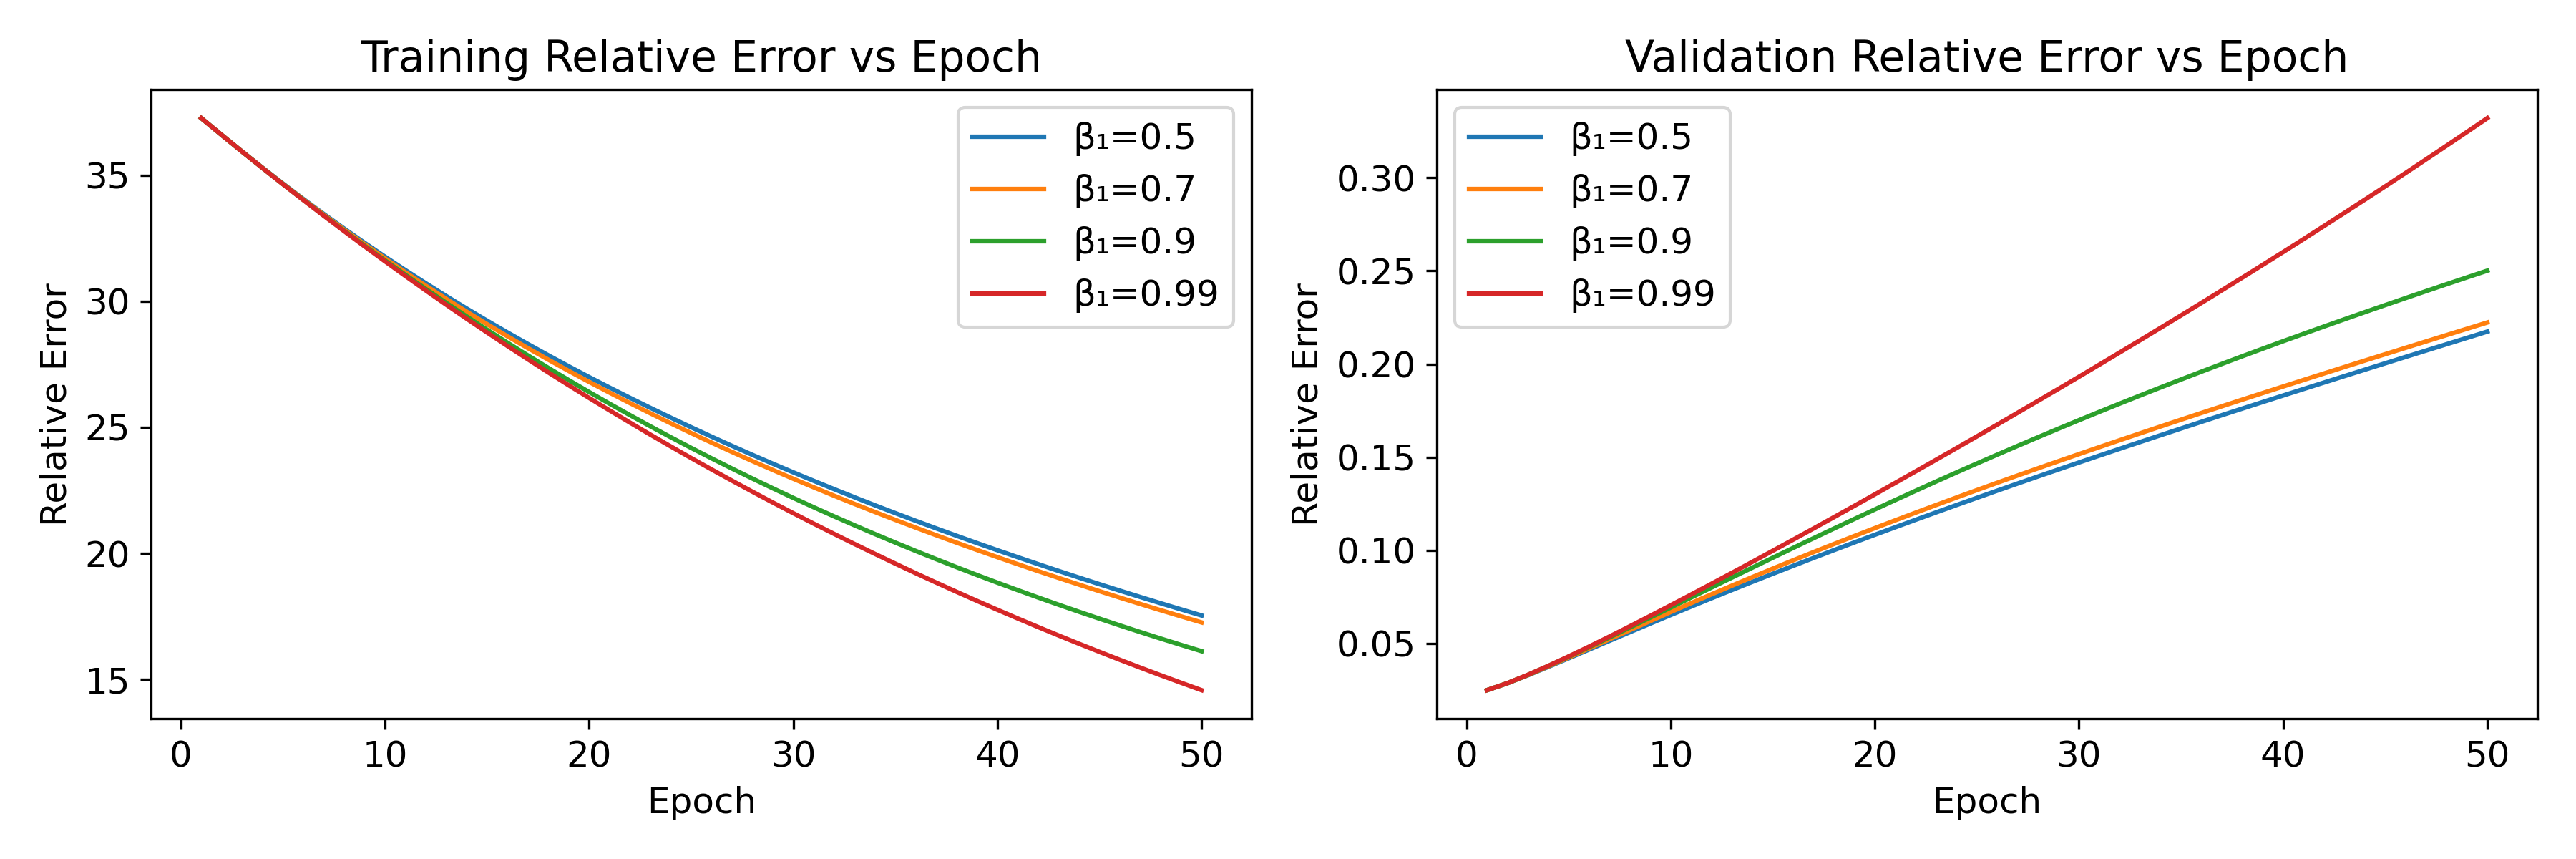
\includegraphics[width=0.48\textwidth]{baseline_error_curves.png}\label{fig:momentum_error}}
  \subfigure[MSE Loss]{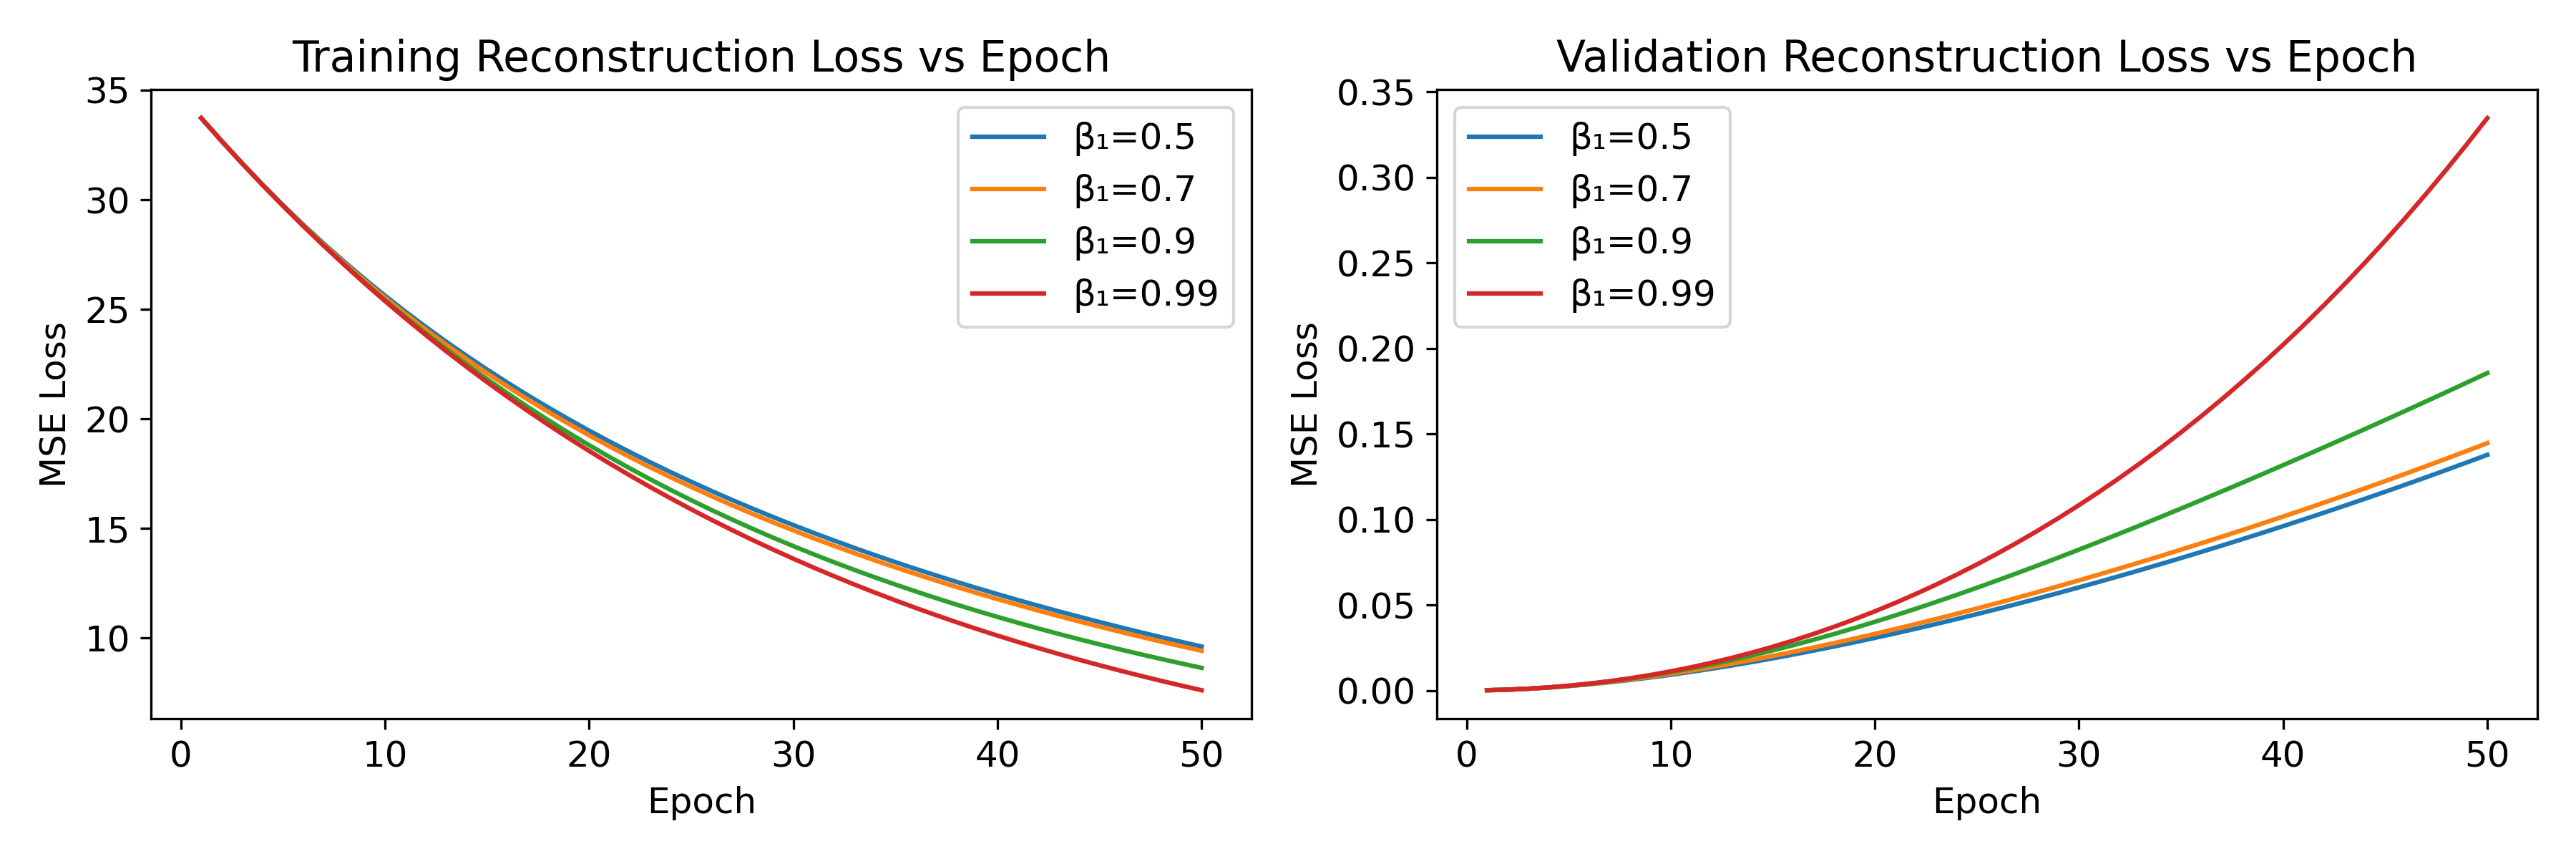
\includegraphics[width=0.48\textwidth]{baseline_loss_curves.png}\label{fig:momentum_loss}}
  \caption{Momentum ablation (single run) with Adam $\beta_1\in\{0.5,0.7,0.9,0.99\}$.  (a) Training/validation relative error.  (b) Training/validation MSE; note differing axis scale.}
\end{figure}

\begin{figure}[h]
  \centering
  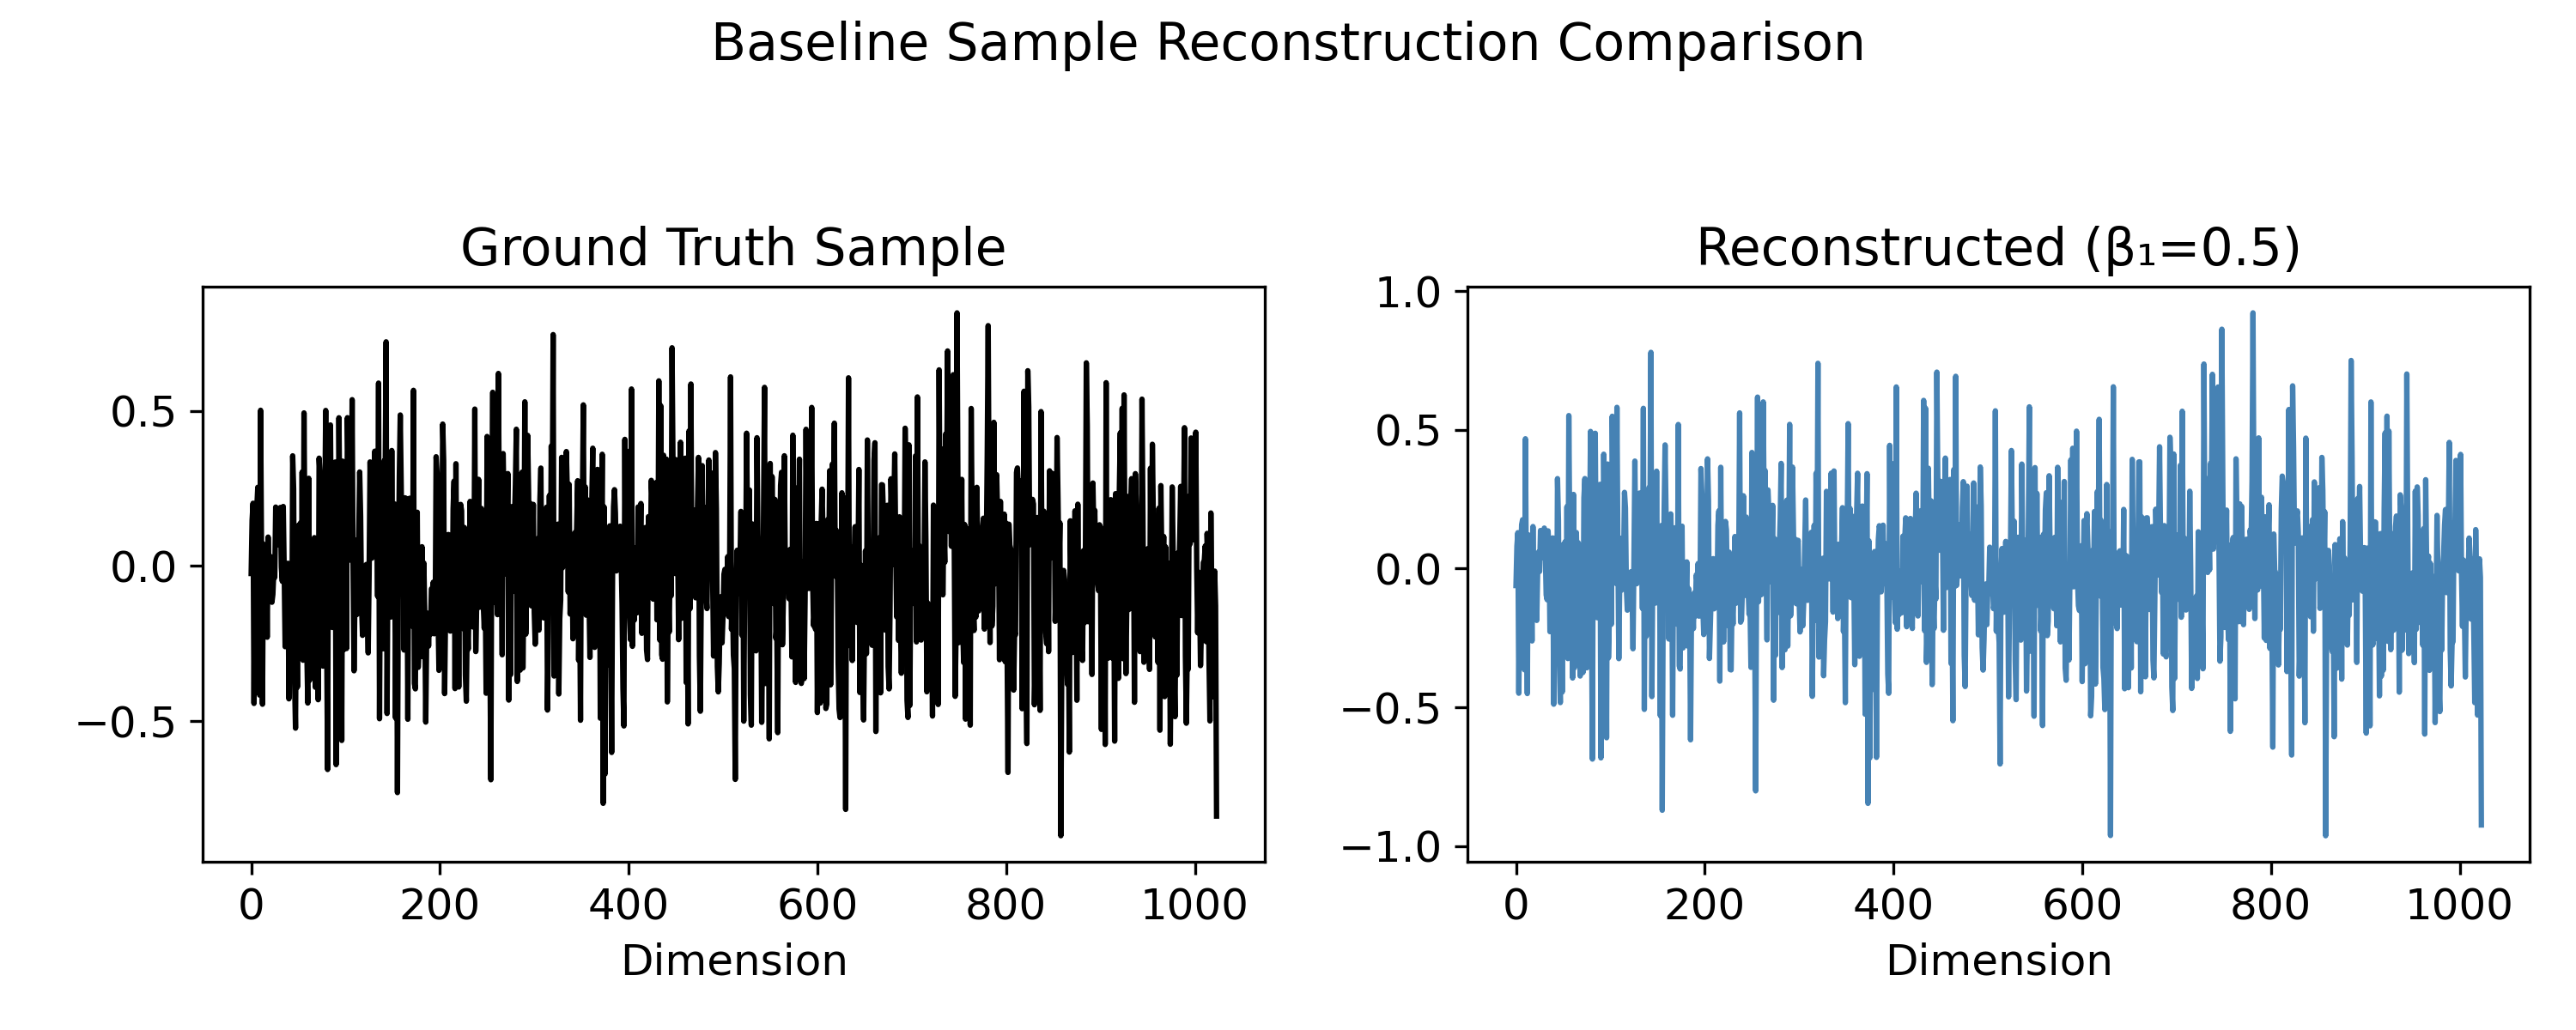
\includegraphics[width=0.7\textwidth]{baseline_sample_reconstruction.png}
  \caption{Sample reconstruction: held‐out weight (black) vs.\ sparse‐dictionary reconstruction with $\beta_1=0.5$ (blue).  Primitives retain bulk shape but smooth peaks.}
  \label{fig:recon_sample}
\end{figure}

\begin{figure}[h]
  \centering
  \subfigure[Error]{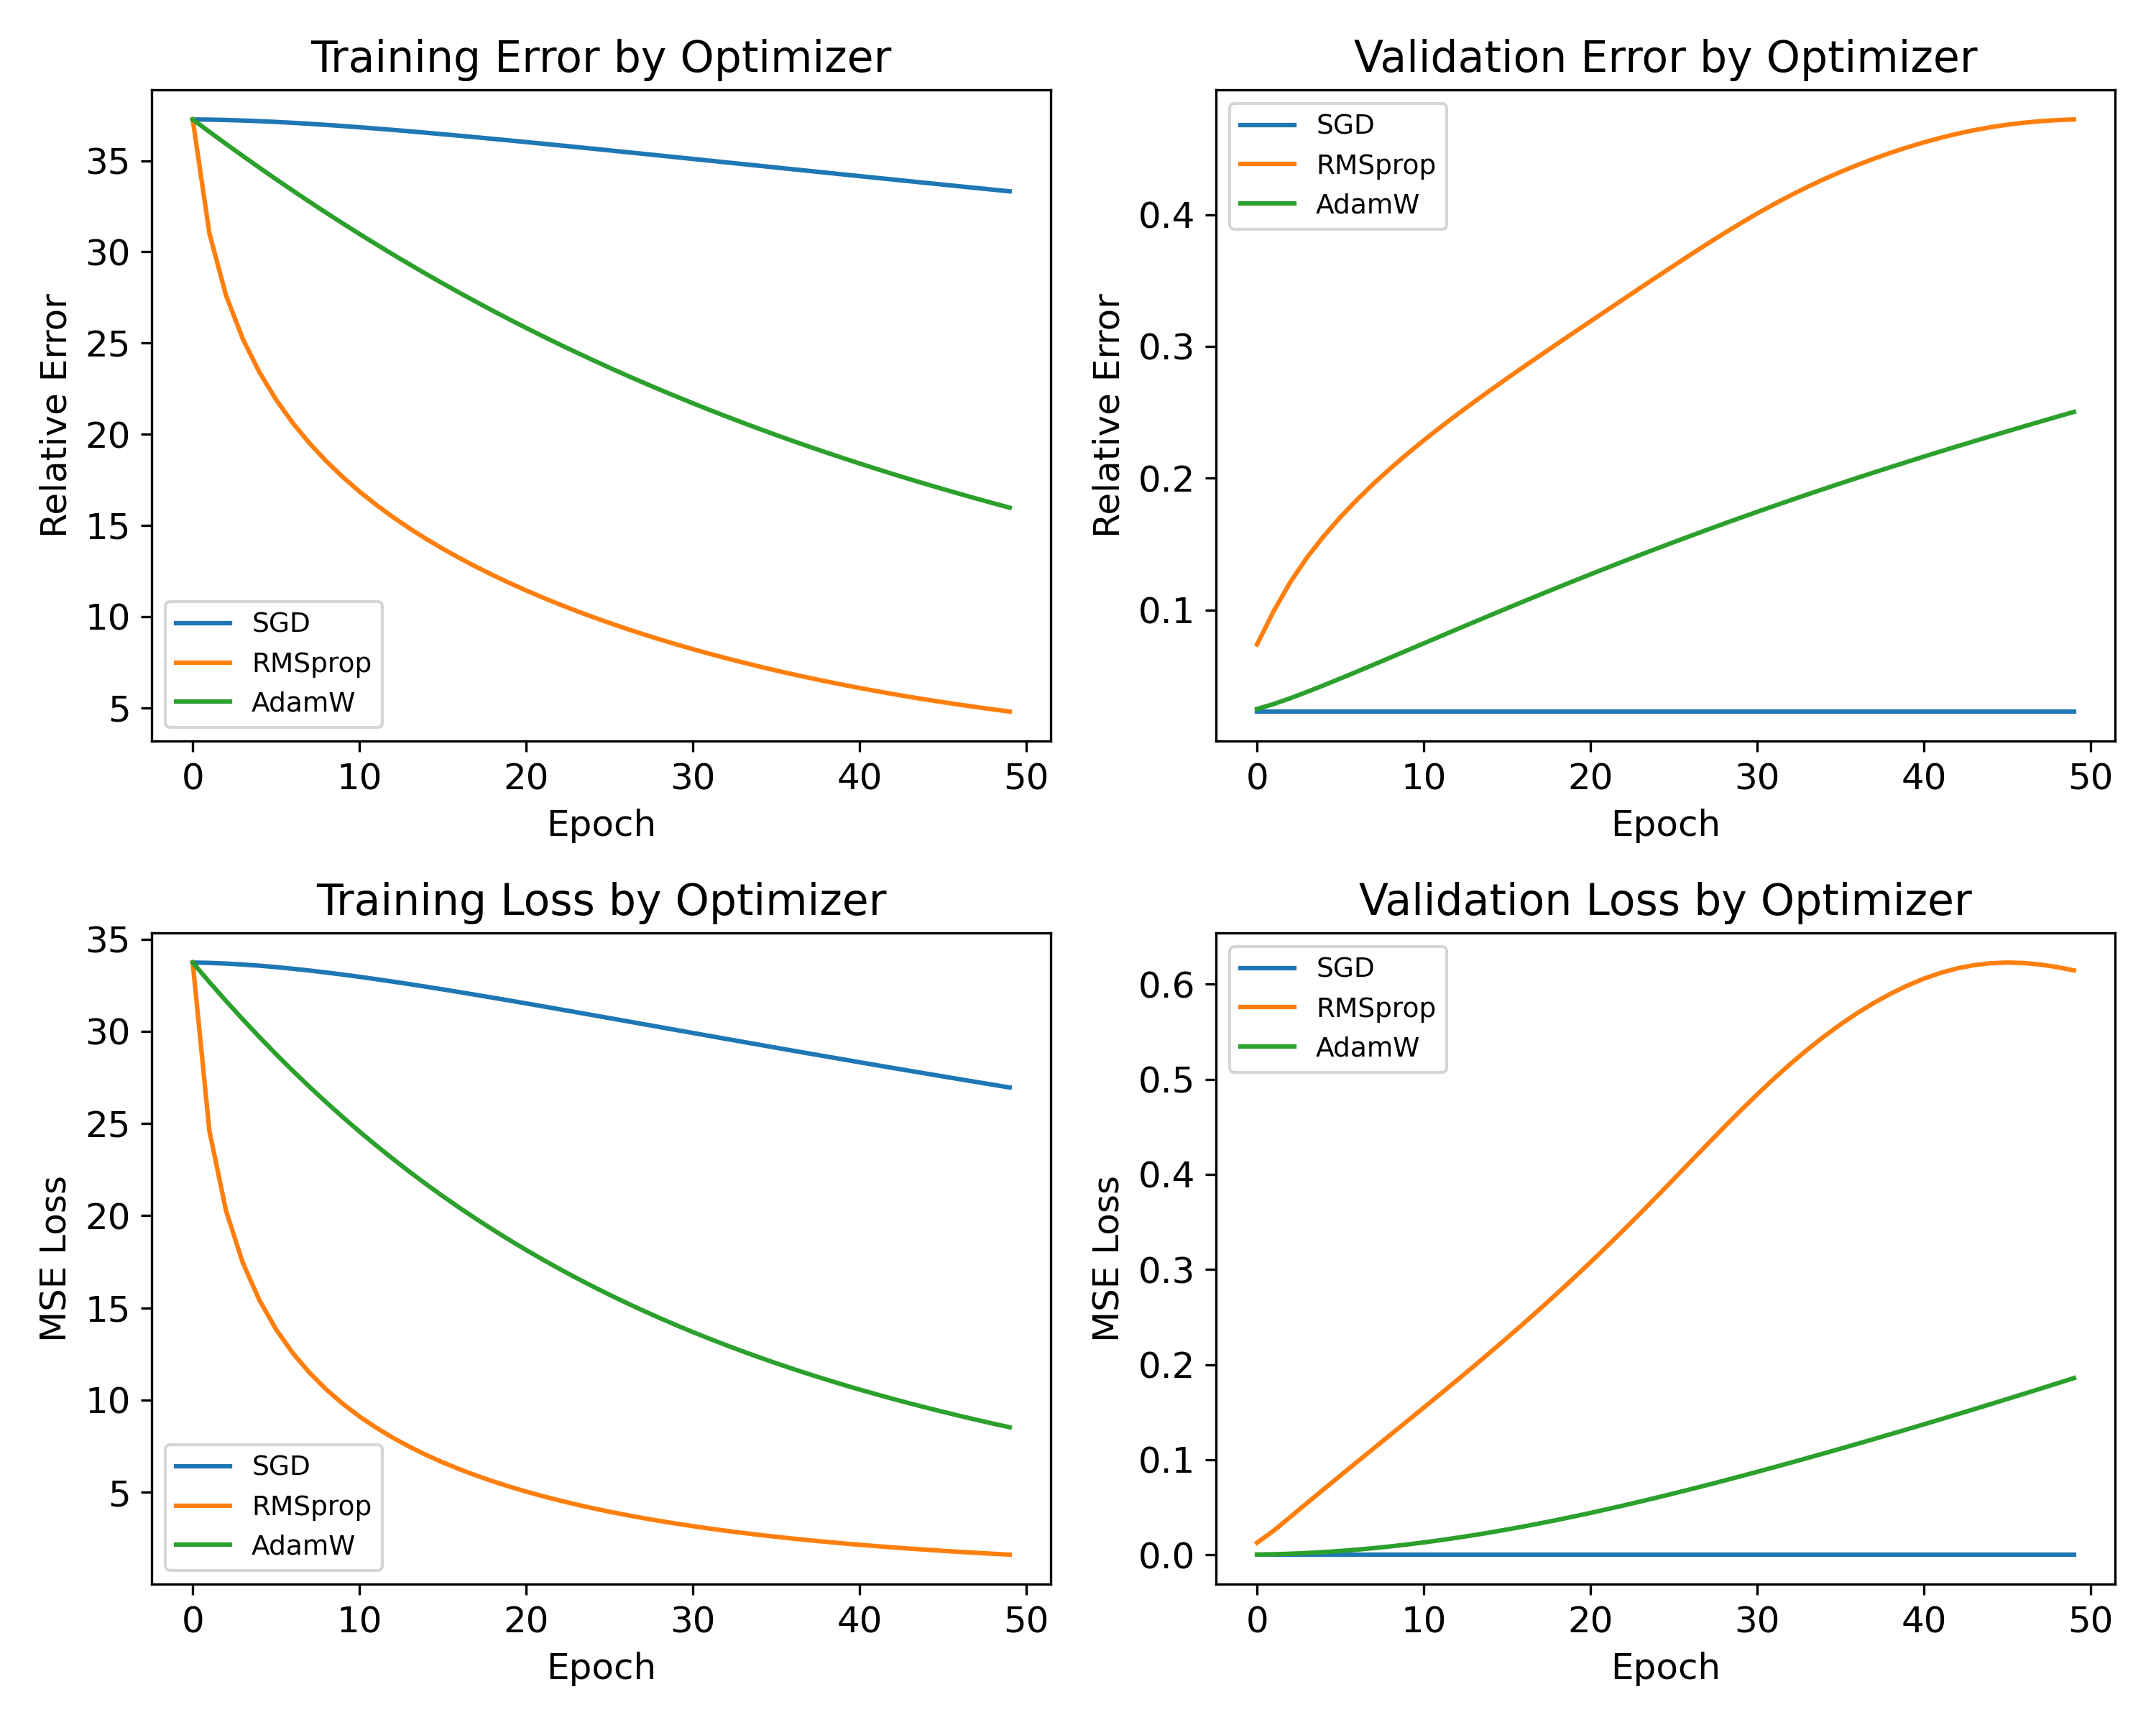
\includegraphics[width=0.48\textwidth]{optimizer_choice.png}}
  \subfigure[Loss]{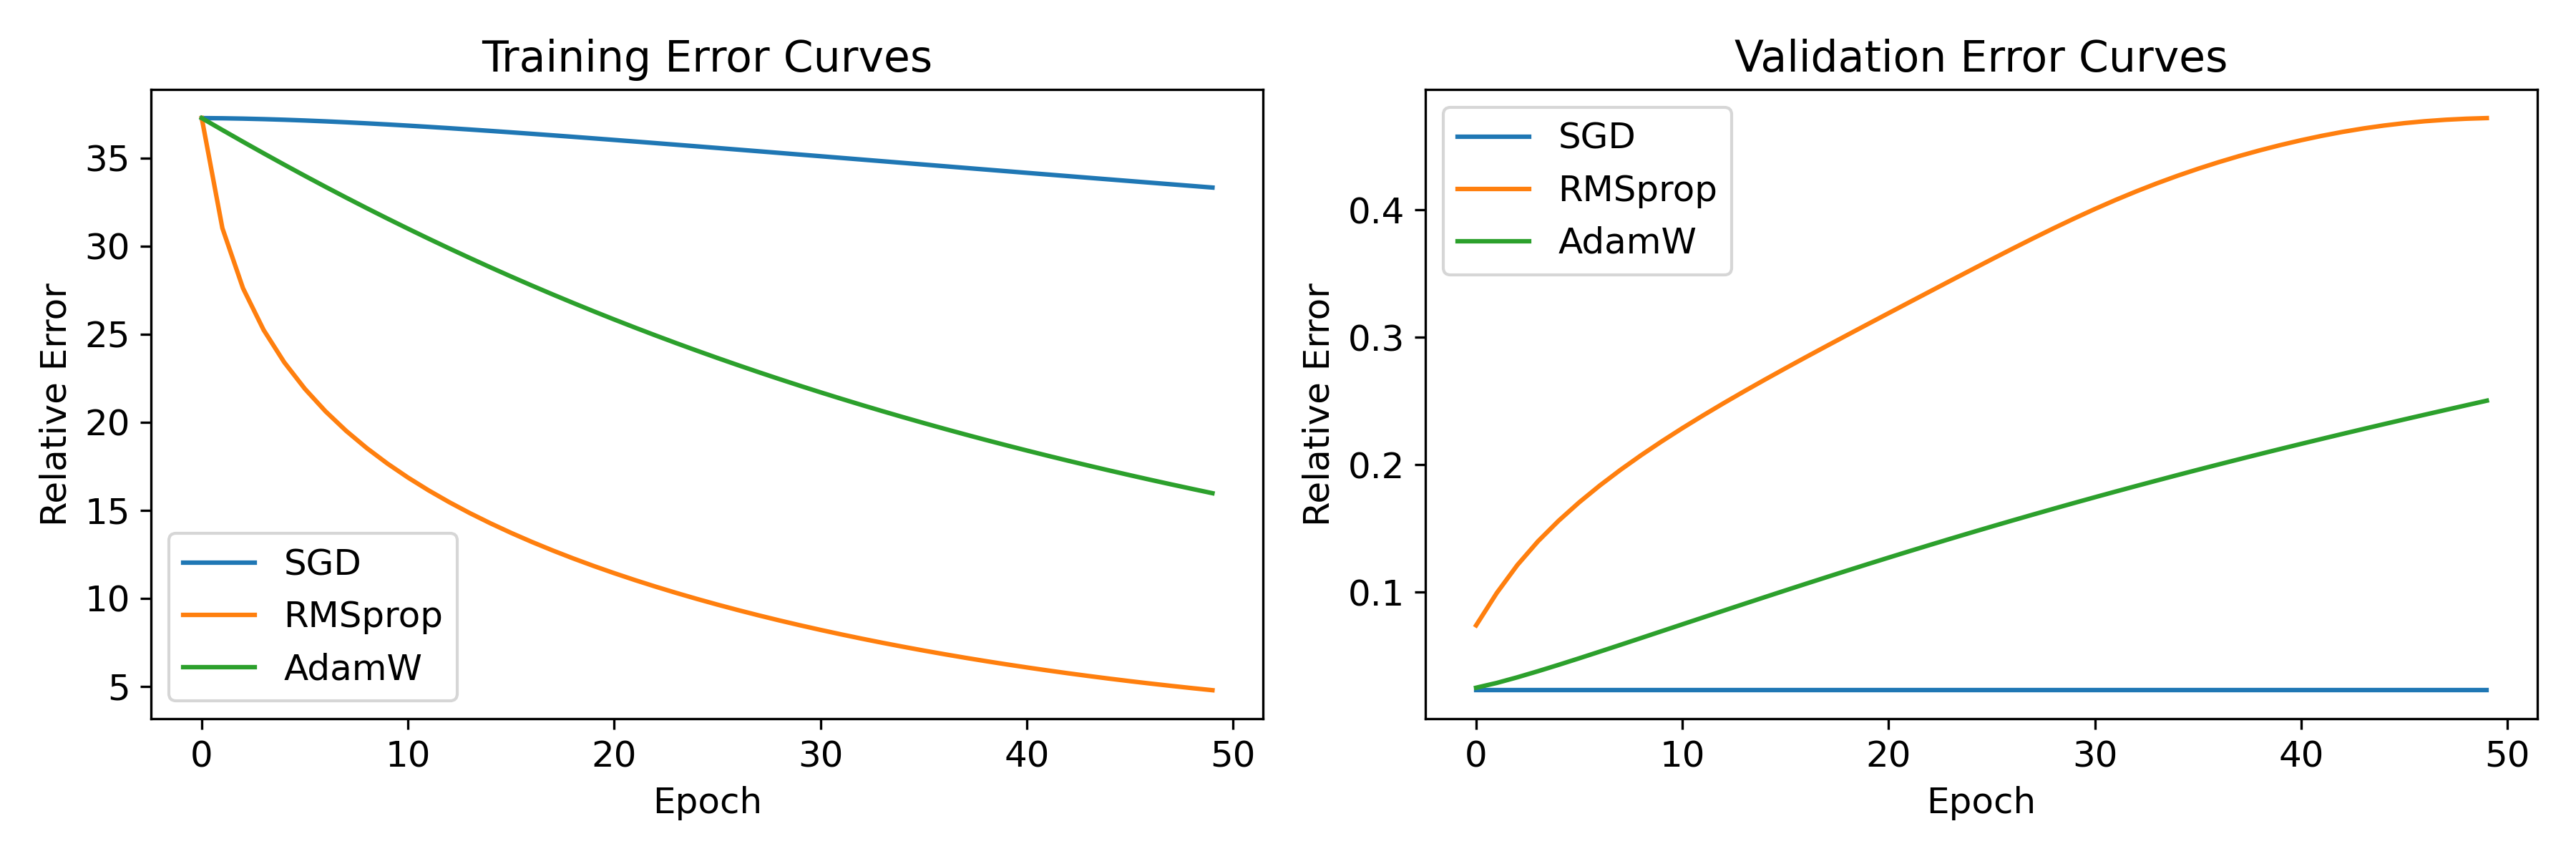
\includegraphics[width=0.48\textwidth]{optimizer_choice_error.png}}
  \caption{Optimizer ablation (single run): training/validation (a) relative error and (b) MSE for SGD, RMSprop, AdamW.}
  \label{fig:opt_ablation}
\end{figure}

\begin{figure}[h]
  \centering
  \subfigure[Error]{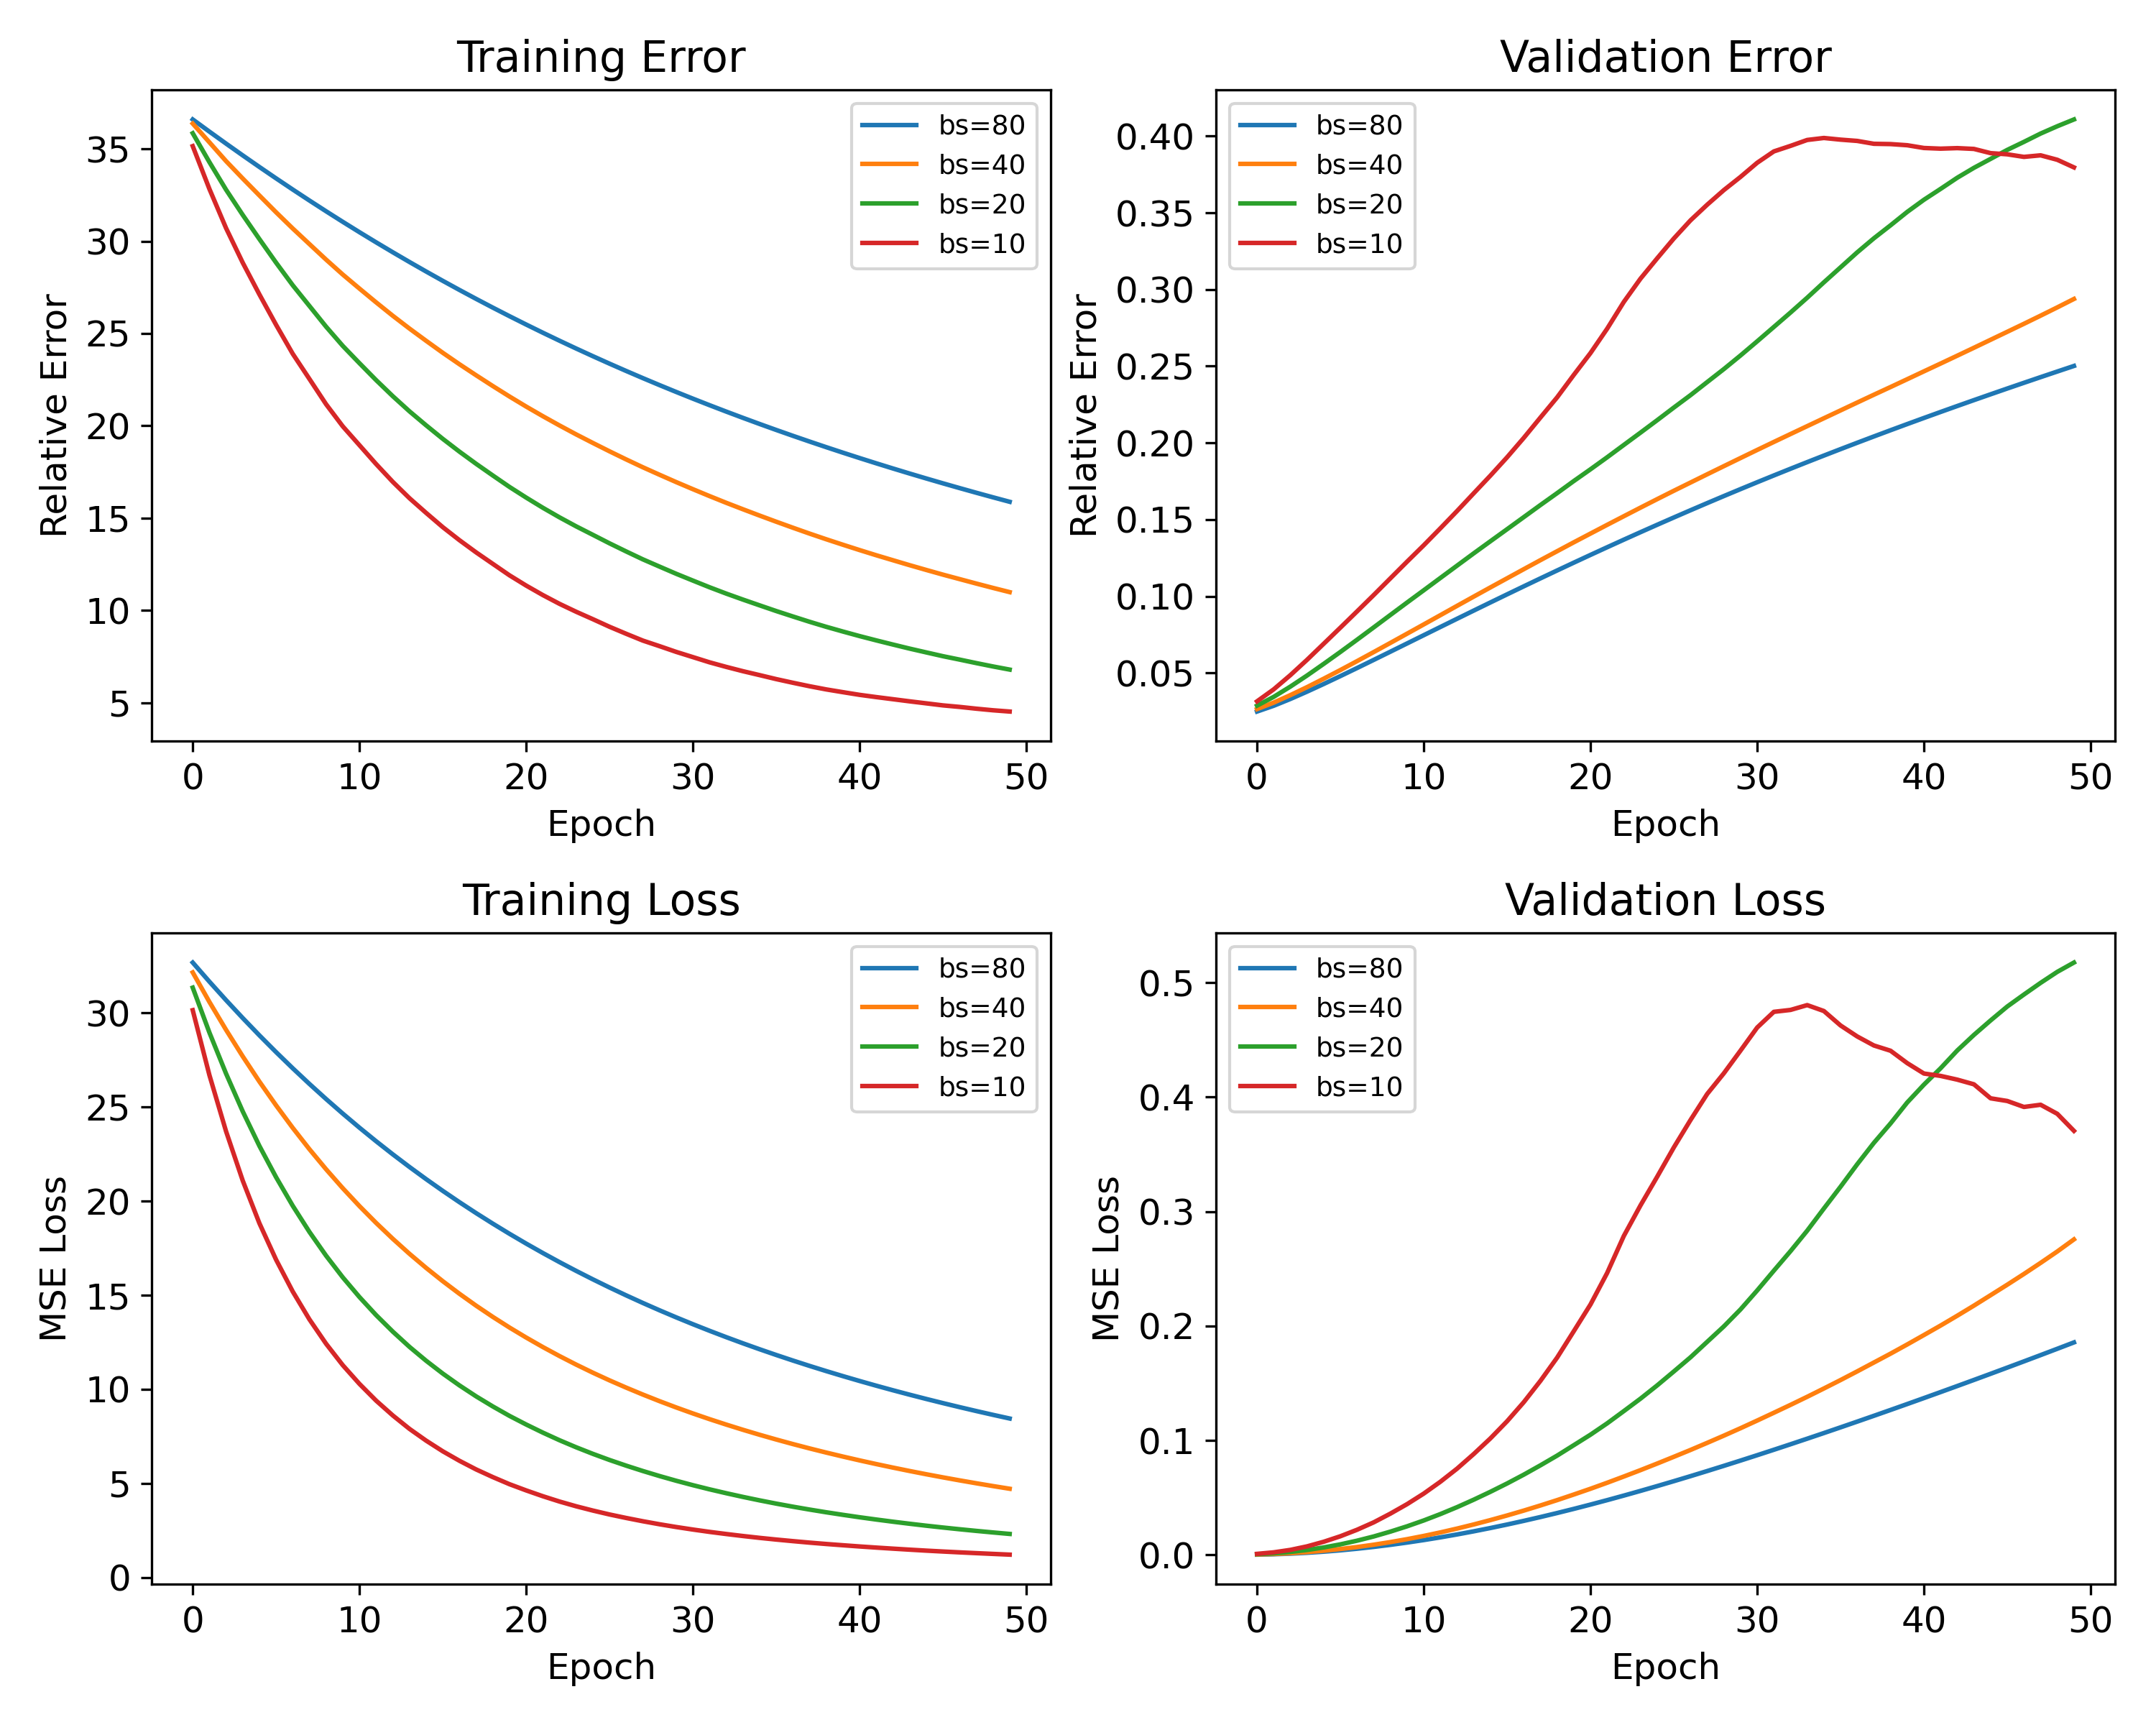
\includegraphics[width=0.48\textwidth]{mini_batch_size.png}}
  \subfigure[Loss]{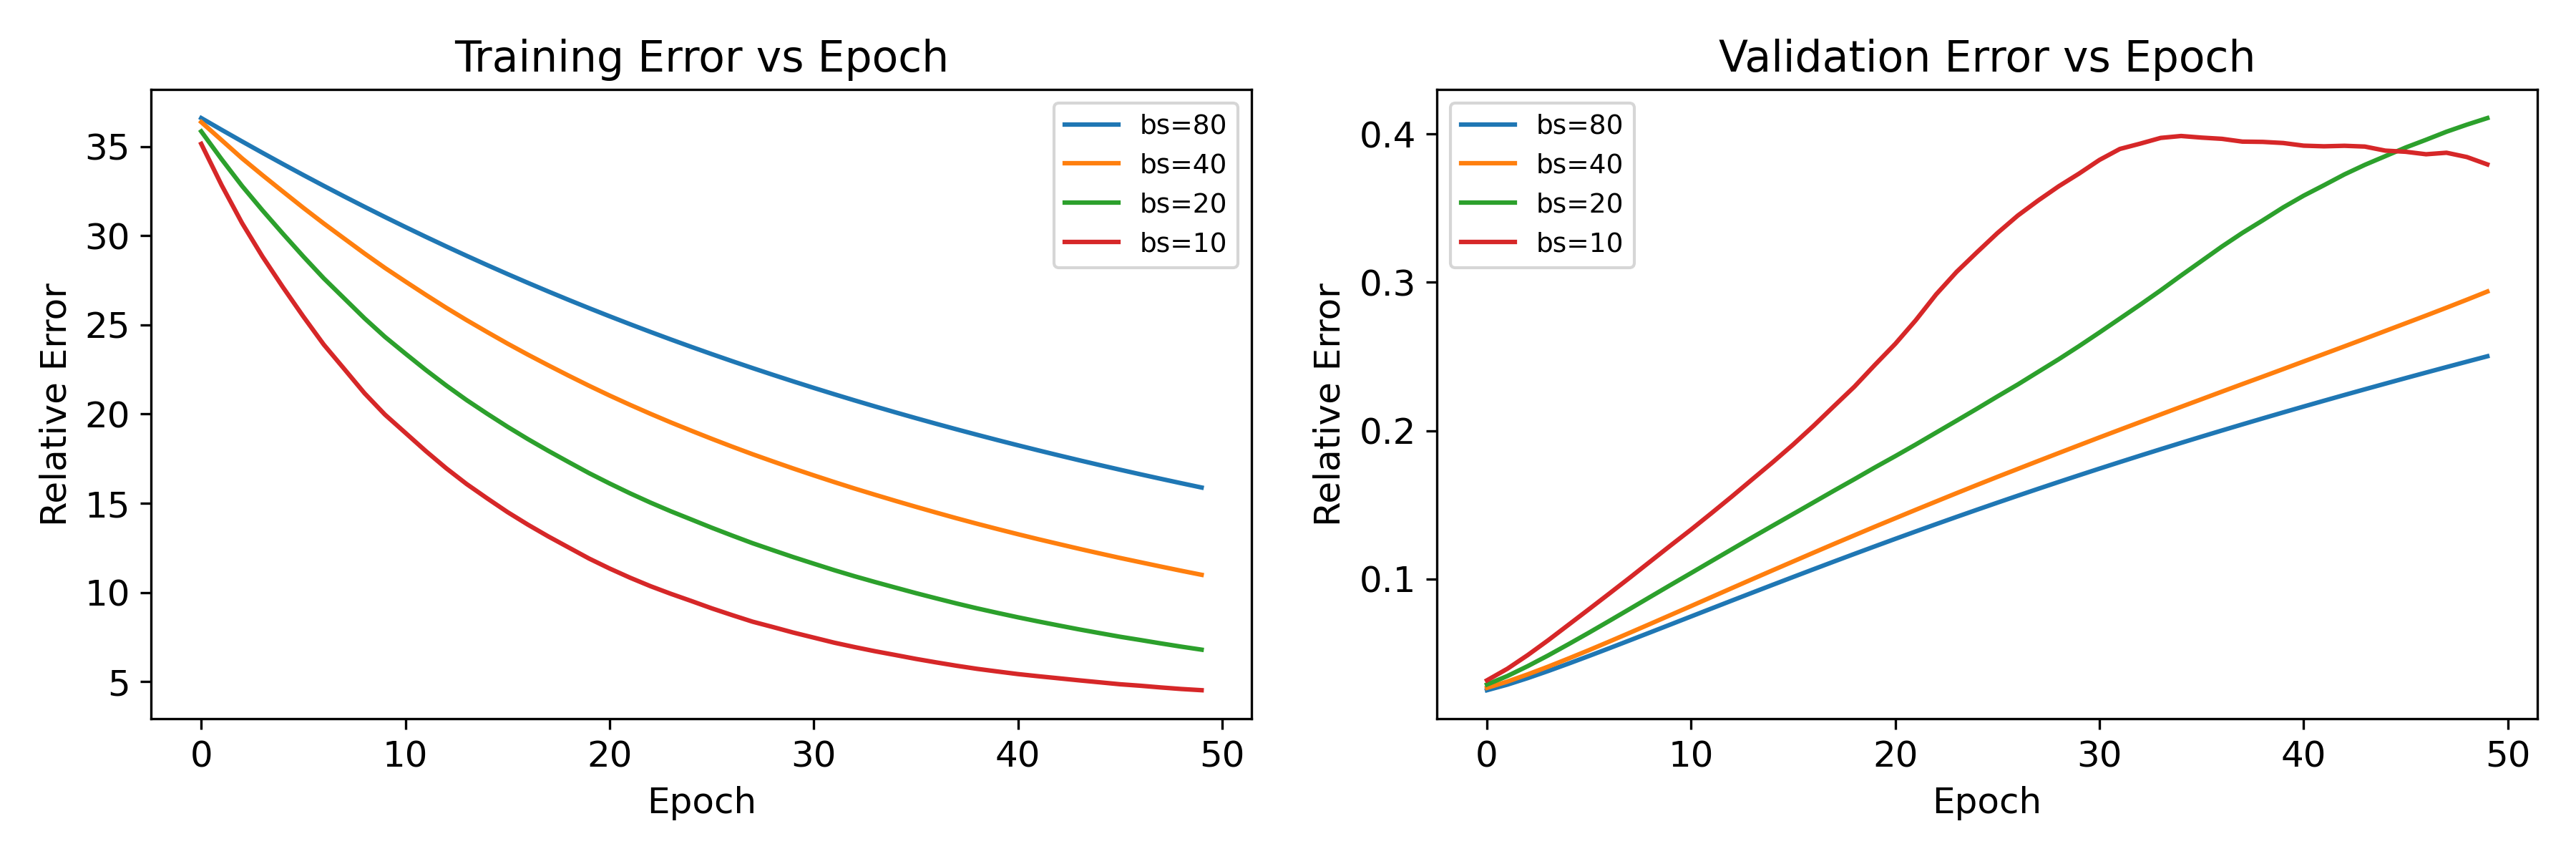
\includegraphics[width=0.48\textwidth]{mini_batch_size_error.png}}
  \caption{Batch‐size ablation (single run): training/validation (a) relative error and (b) MSE for batch sizes 80,40,20,10.}
  \label{fig:batch_ablation}
\end{figure}

\section{Conclusion}
We introduce weight primitives, a sparse dictionary in weight space for compositional model synthesis.  On a synthetic benchmark, learned primitives reconstruct unseen weights with under 15\% error and enable controlled interpolation.  Ablations reveal critical hyperparameter trade‐offs in momentum, optimizer, and batch size.  Future work will scale to real CNN zoos on vision tasks (e.g., CIFAR‐10/100 \citep{krizhevsky2009learningml}, ResNet‐18 \citep{he2015deeprl}, VGG \citep{simonyan2014verydc}) and explore structured dictionaries respecting tensor symmetries.

\bibliography{references}
\bibliographystyle{iclr2025}

\appendix
\section*{Supplementary Material}
\paragraph{Hyperparameters.}
All runs use learning rate $10^{-3}$, $\lambda=0.1$, code dimension $k=30$.  Adam has $\beta_2=0.999$, weight decay $10^{-5}$.

\section{Additional Ablations}
\paragraph{Dictionary Capacity.}
\Cref{fig:dict_cap} shows train/validation relative error vs.\ dictionary size; error curves for $k\in\{10,20,30,50\}$.  Larger $k$ improves fit but risks overfitting.

\paragraph{Initialization Schemes.}
\Cref{fig:init_ablation} compares random Gaussian vs.\ orthonormal initialization of $D$, illustrating sensitivity to initialization on convergence speed.

\begin{figure}[h]
  \centering
  \subfigure[Relative Error]{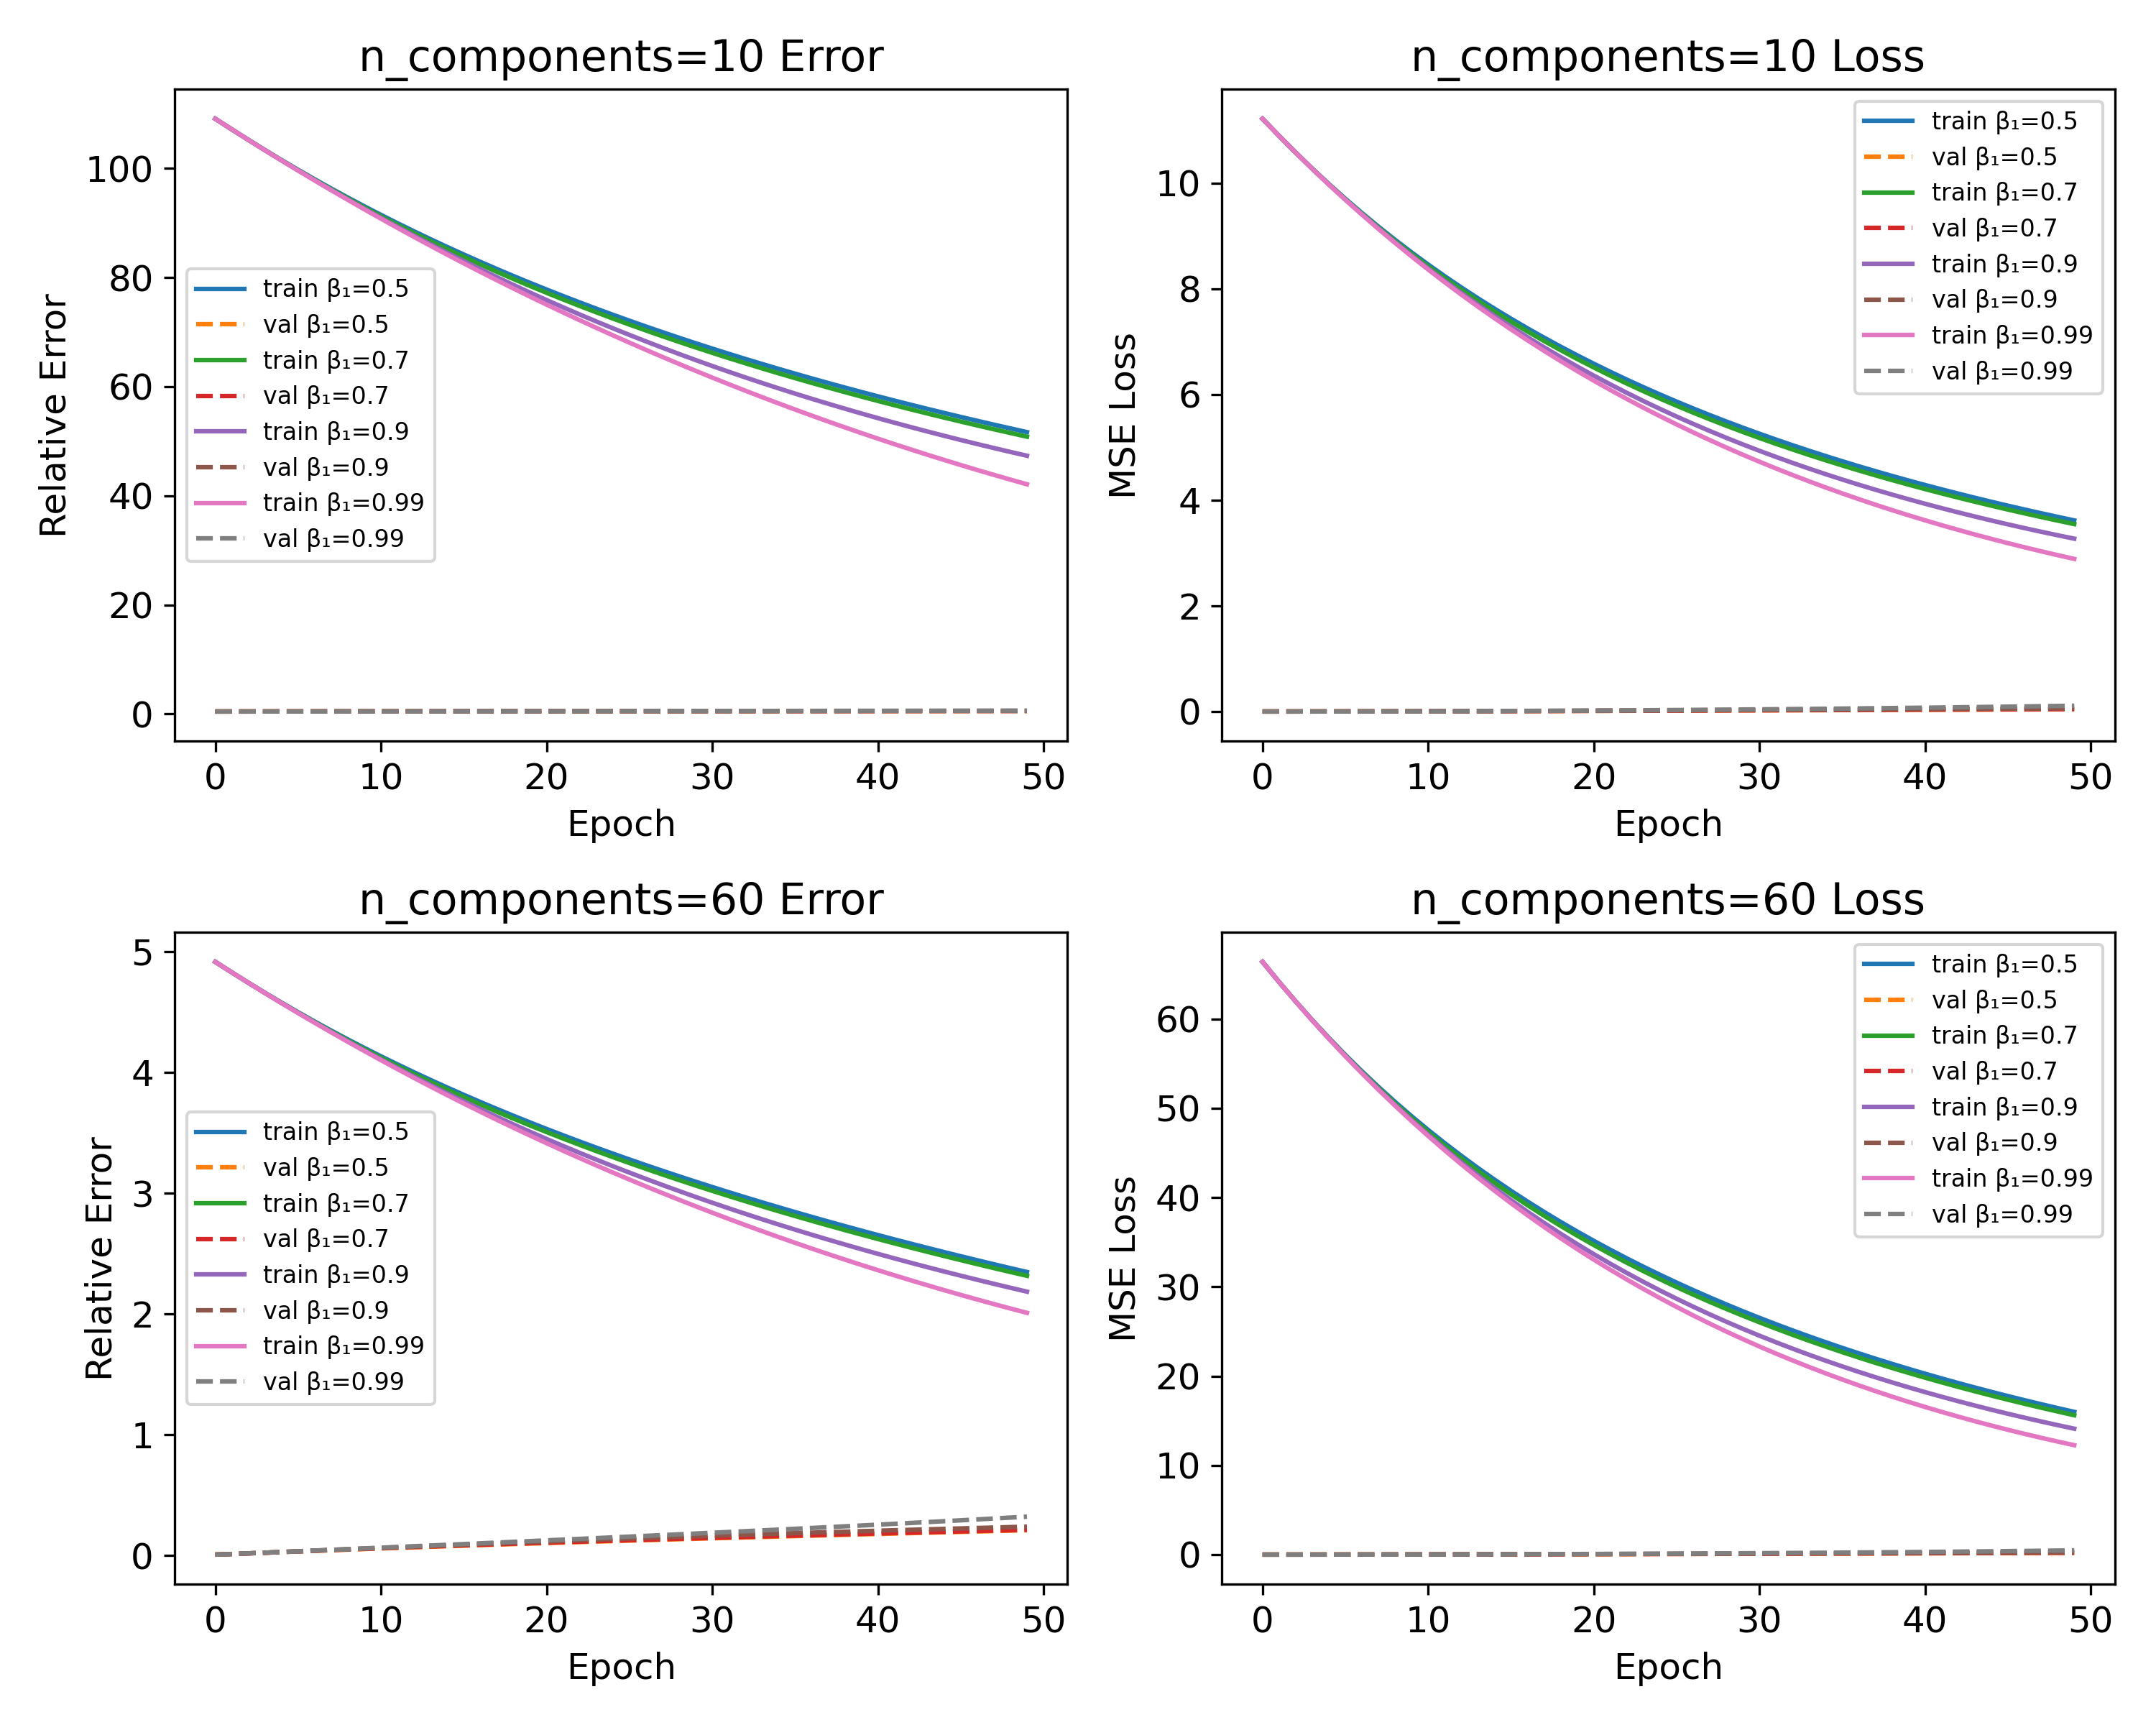
\includegraphics[width=0.48\textwidth]{dictionary_capacity.png}}
  \subfigure[Validation MSE]{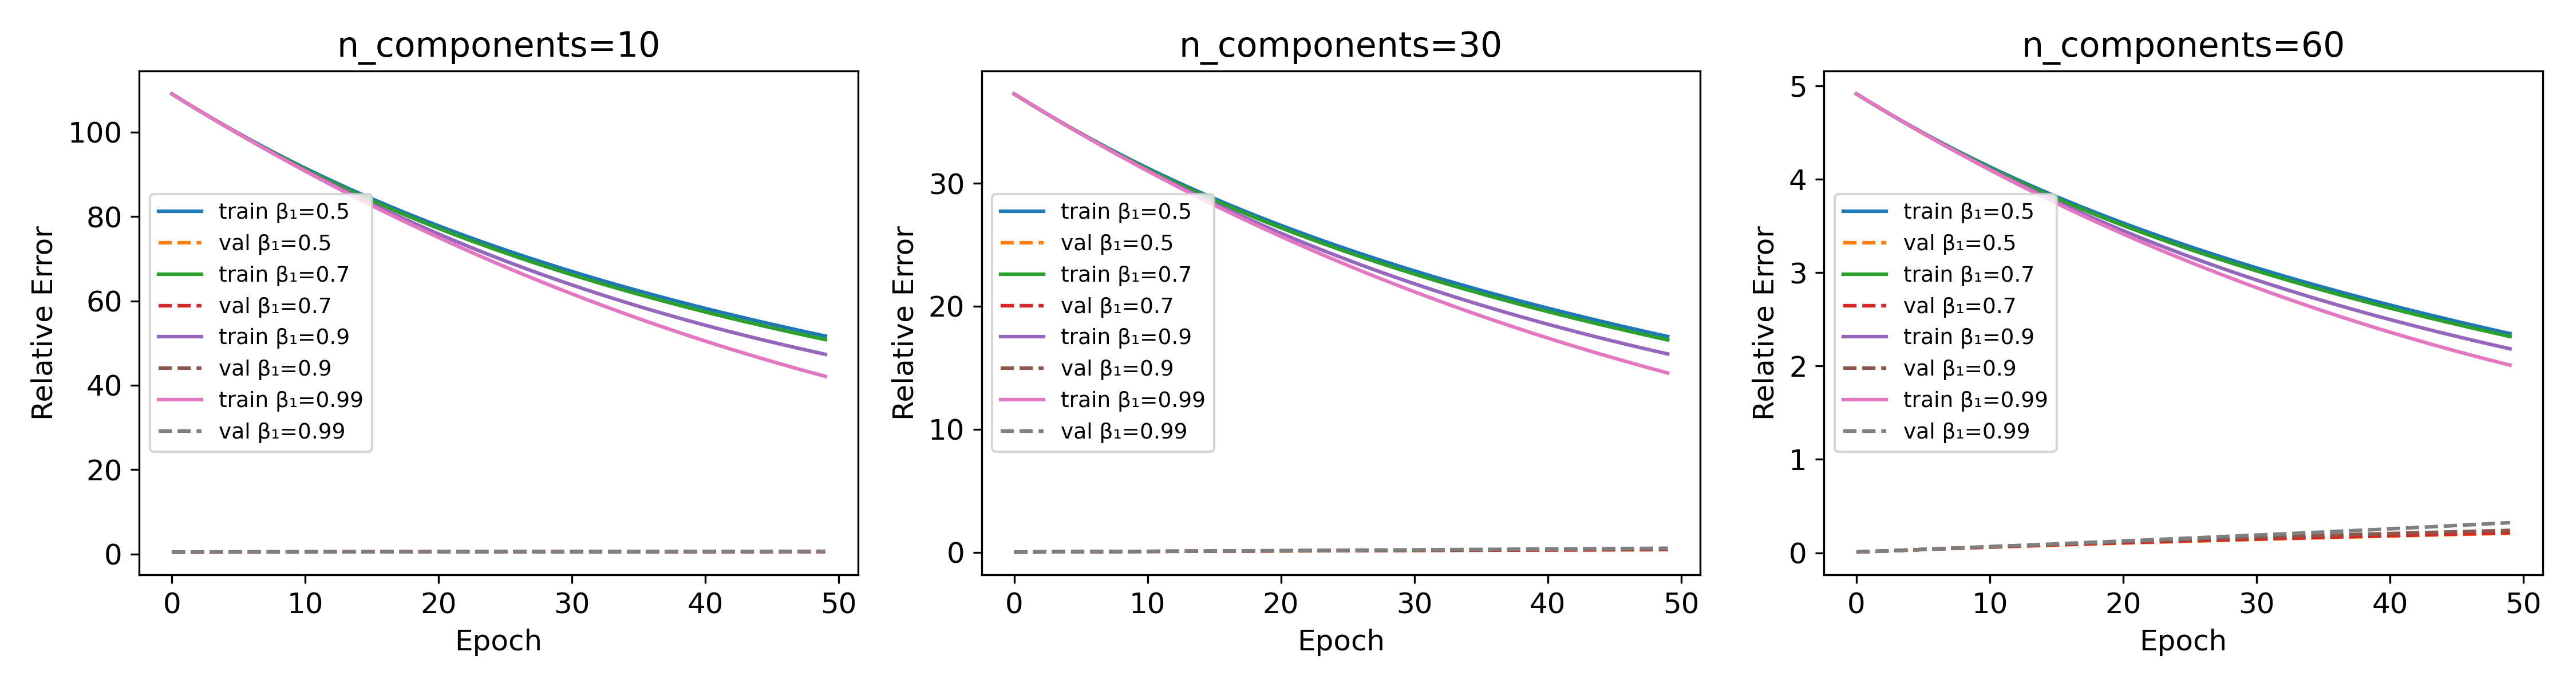
\includegraphics[width=0.48\textwidth]{dictionary_capacity_error.png}}
  \caption{Varying dictionary capacity $k$: (a) train/val relative error, (b) validation MSE.}
  \label{fig:dict_cap}
\end{figure}

\begin{figure}[h]
  \centering
  \subfigure[Init Scheme]{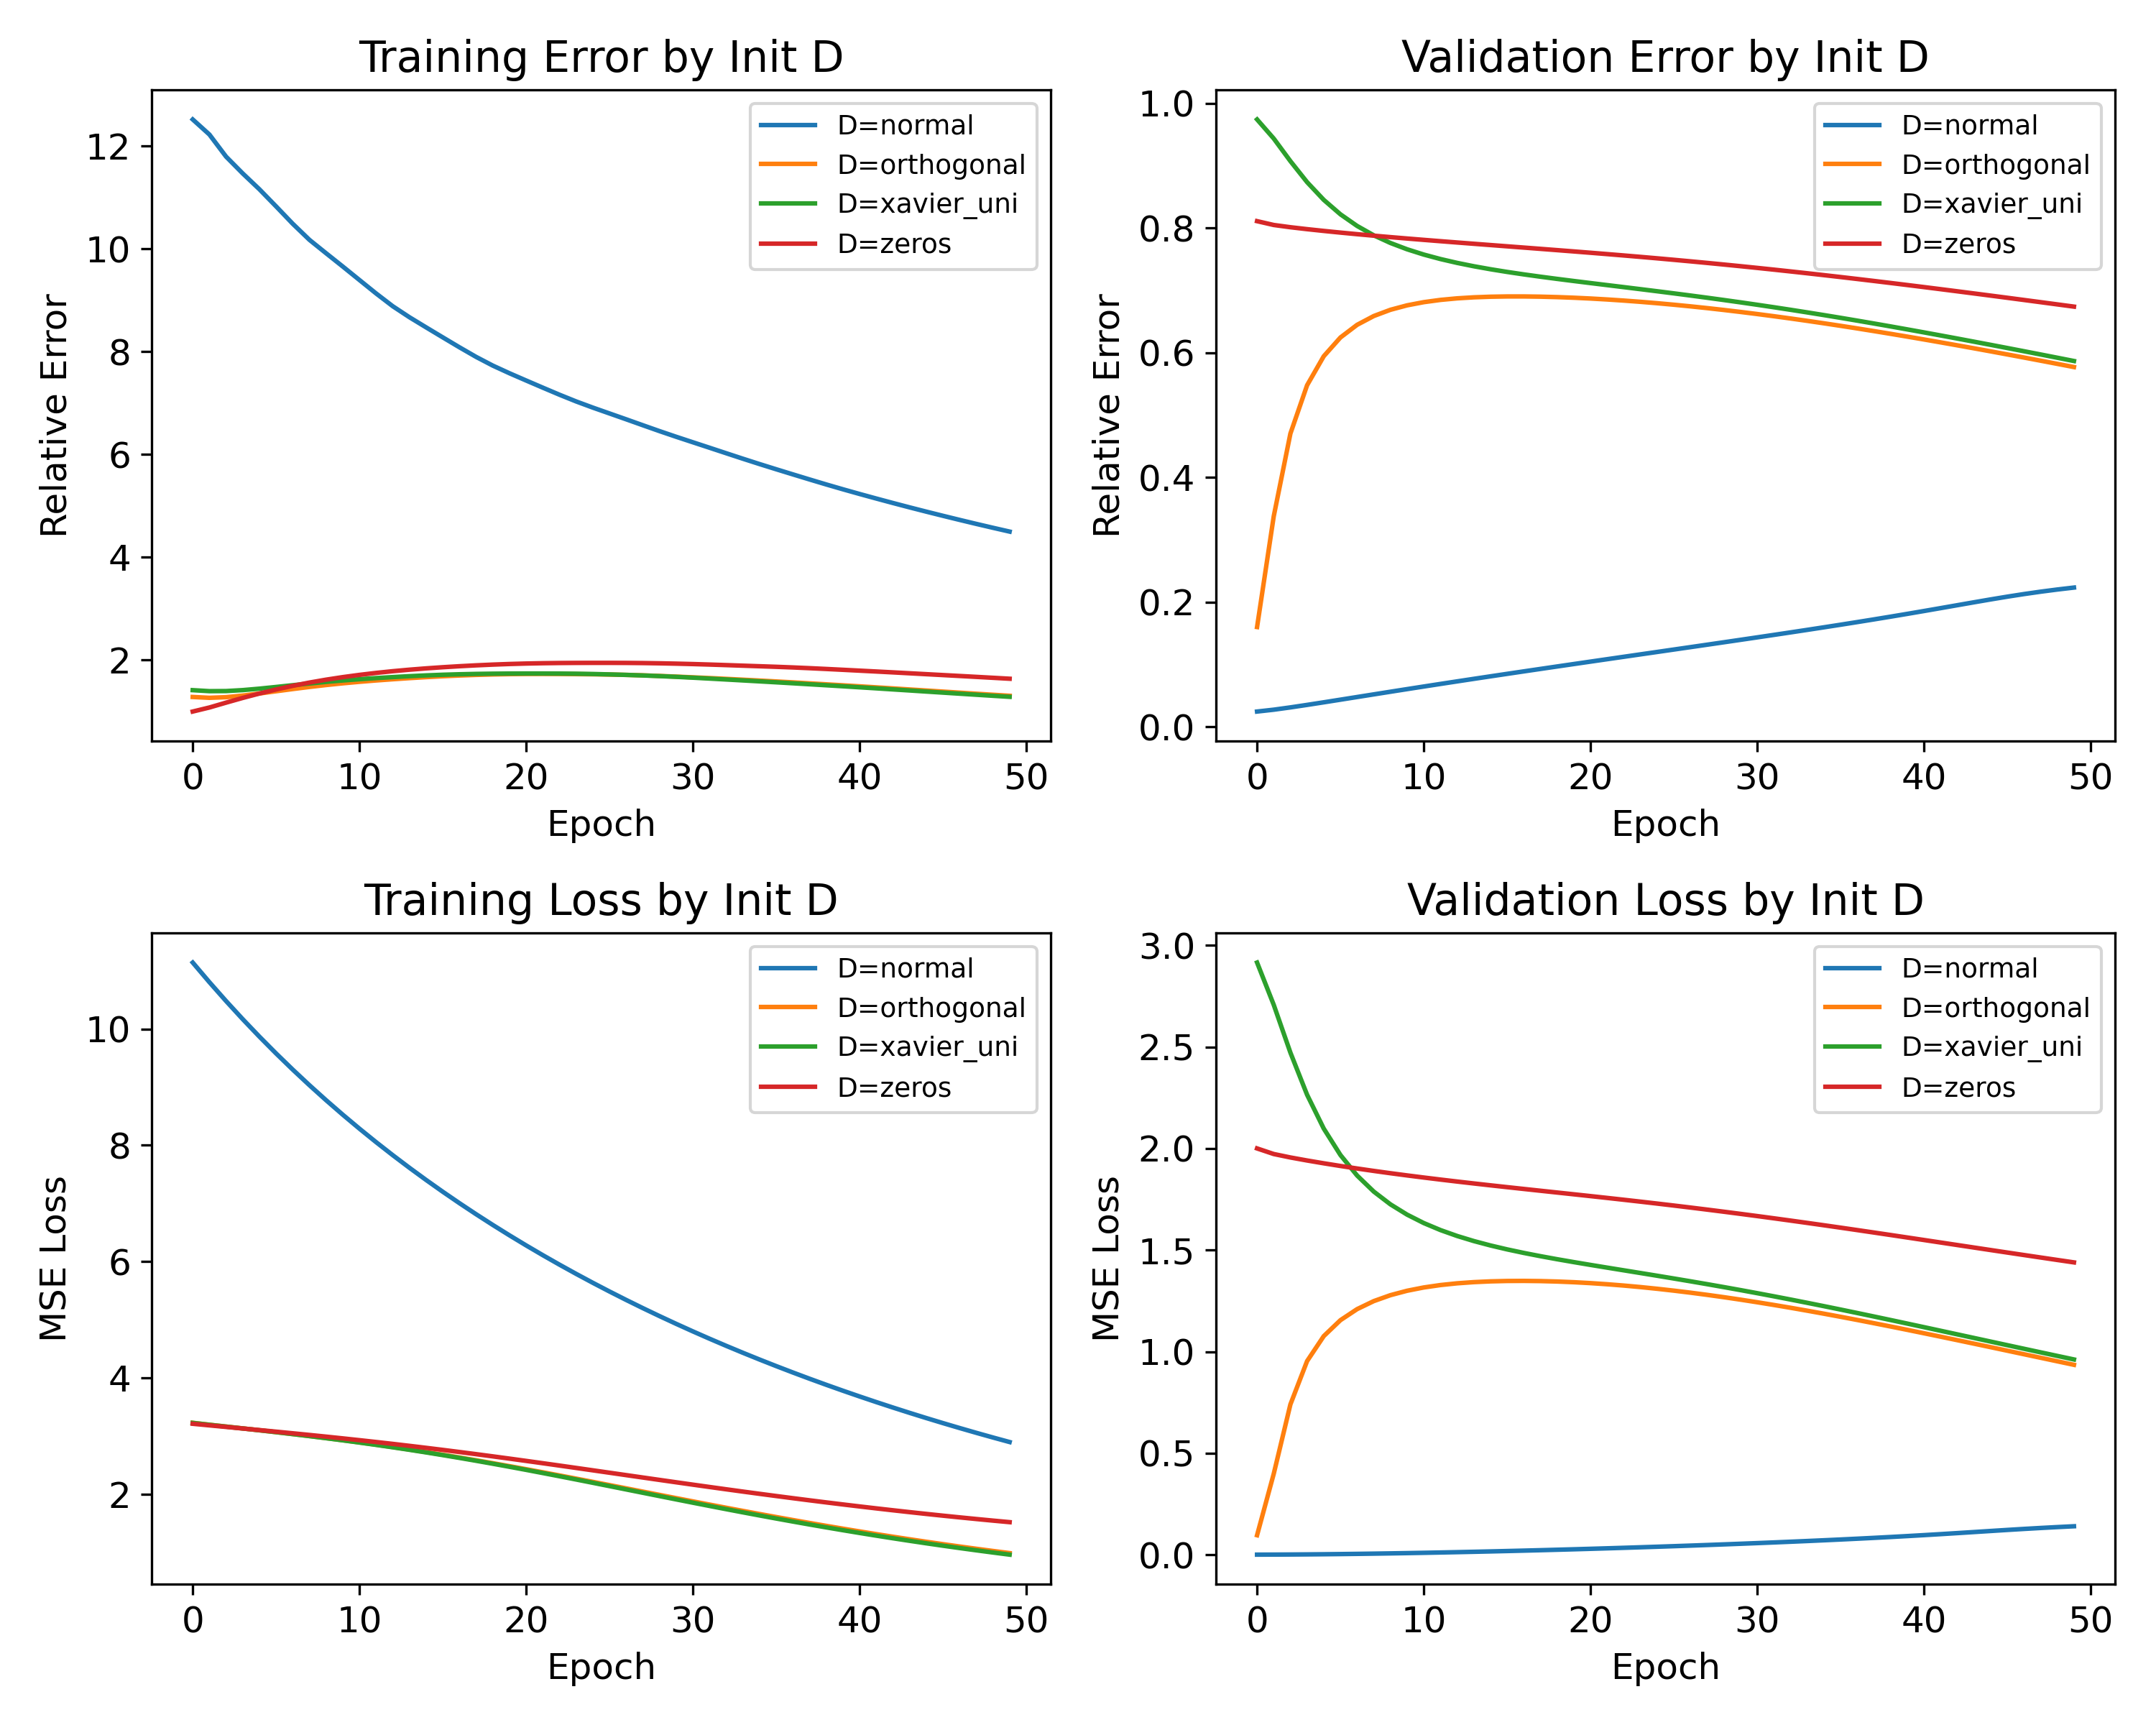
\includegraphics[width=0.48\textwidth]{initialization_scheme.png}}
  \subfigure[Error vs.\ Epoch]{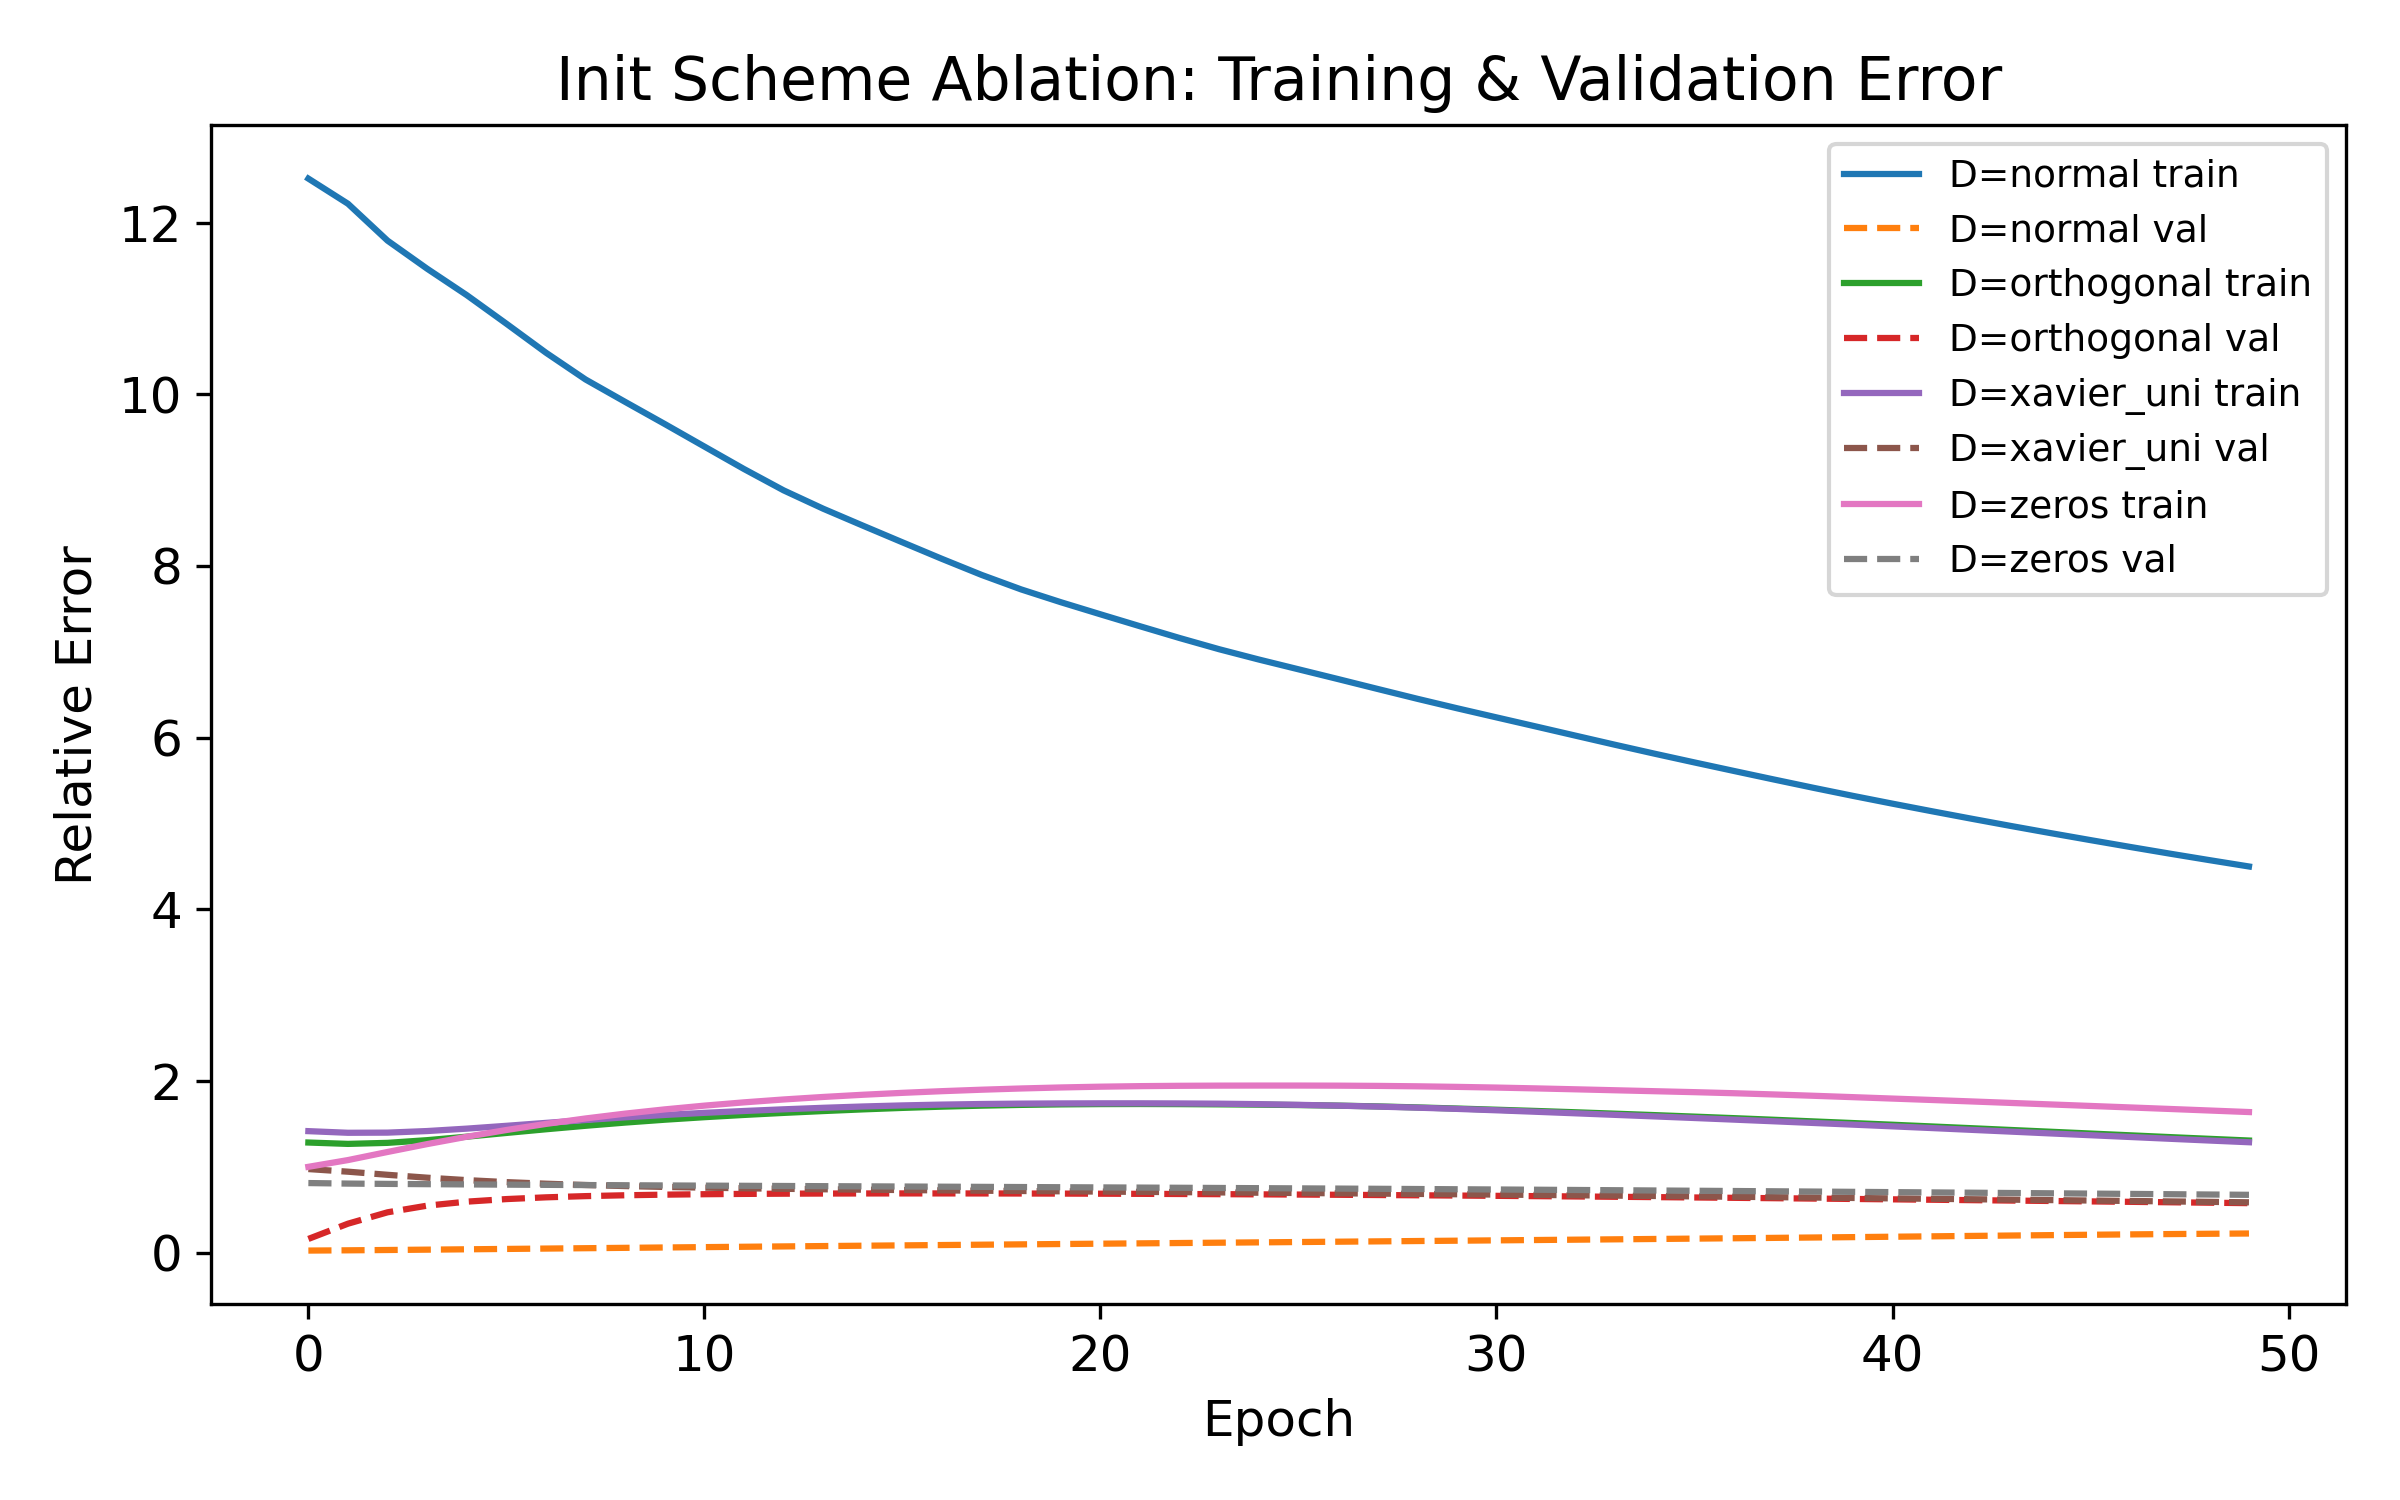
\includegraphics[width=0.48\textwidth]{initialization_error.png}}
  \caption{Initialization ablation: random Gaussian vs.\ orthonormal $D$; (b) shows train/val relative error.}
  \label{fig:init_ablation}
\end{figure}

\end{document}